\chapter{Tests und Analysen}
\label{sec:analysen}

In diesem Kapitel wird die Leistungsfähigkeit des gesamten Systems evaluiert. Die Beurteilung erfolgt anhand von KI-generierten Videodaten, die dem System während der Trainingsphase nicht präsentiert wurden. Im Fokus steht dabei die Frage, ob die Verbesserungen durch zeitliche Aggregation und die zweistufige Verarbeitungskette zuverlässiger sind als die alleinige Verwendung der Objekterkennung und Segmentierung. Dabei ist es interessant zu sehen, in welchen Szenarien diese Zusätze das System deutlich beeinflussen.


\section{Modell-Performance (Training \& Validation)}
Da die YOLO-Modelle einen wesentlichen Teil der Zuverlässigkeit des Systems beeinflussen, werfen wir zuerst einen Blick auf deren isolierte Leistung.

In diesem Unterkapitel wird vor allem auf die Trainingsmetriken eingegangen. Besonders Interessant sind dabei die Verlustfunktionen, welche angeben wie viele Fehler auf den jeweiligen Datensatz (Training oder Validierung) passiert sind. Die Informationen der Wahrheitsmatrizzen geben dabei Einsicht wie viele Objekte erkannt, fälschlicherweise erkannt oder vom Modell erfunden wurden.

\subsection{Leistung der Objekterkennung}
Die Trainingsmetriken (Abbildung \ref{fig:training_det}) für den Katzengesicht-Detektor, zeigen einen kontinuierlich sinkenden Trainingsfehler (\emph{engl. Loss}) und eine hohe Genauigkeit (\emph{engl. Precision}) in der Validierung im Verlauf von 100 Epochen.

\begin{figure}[H]
    \centering
    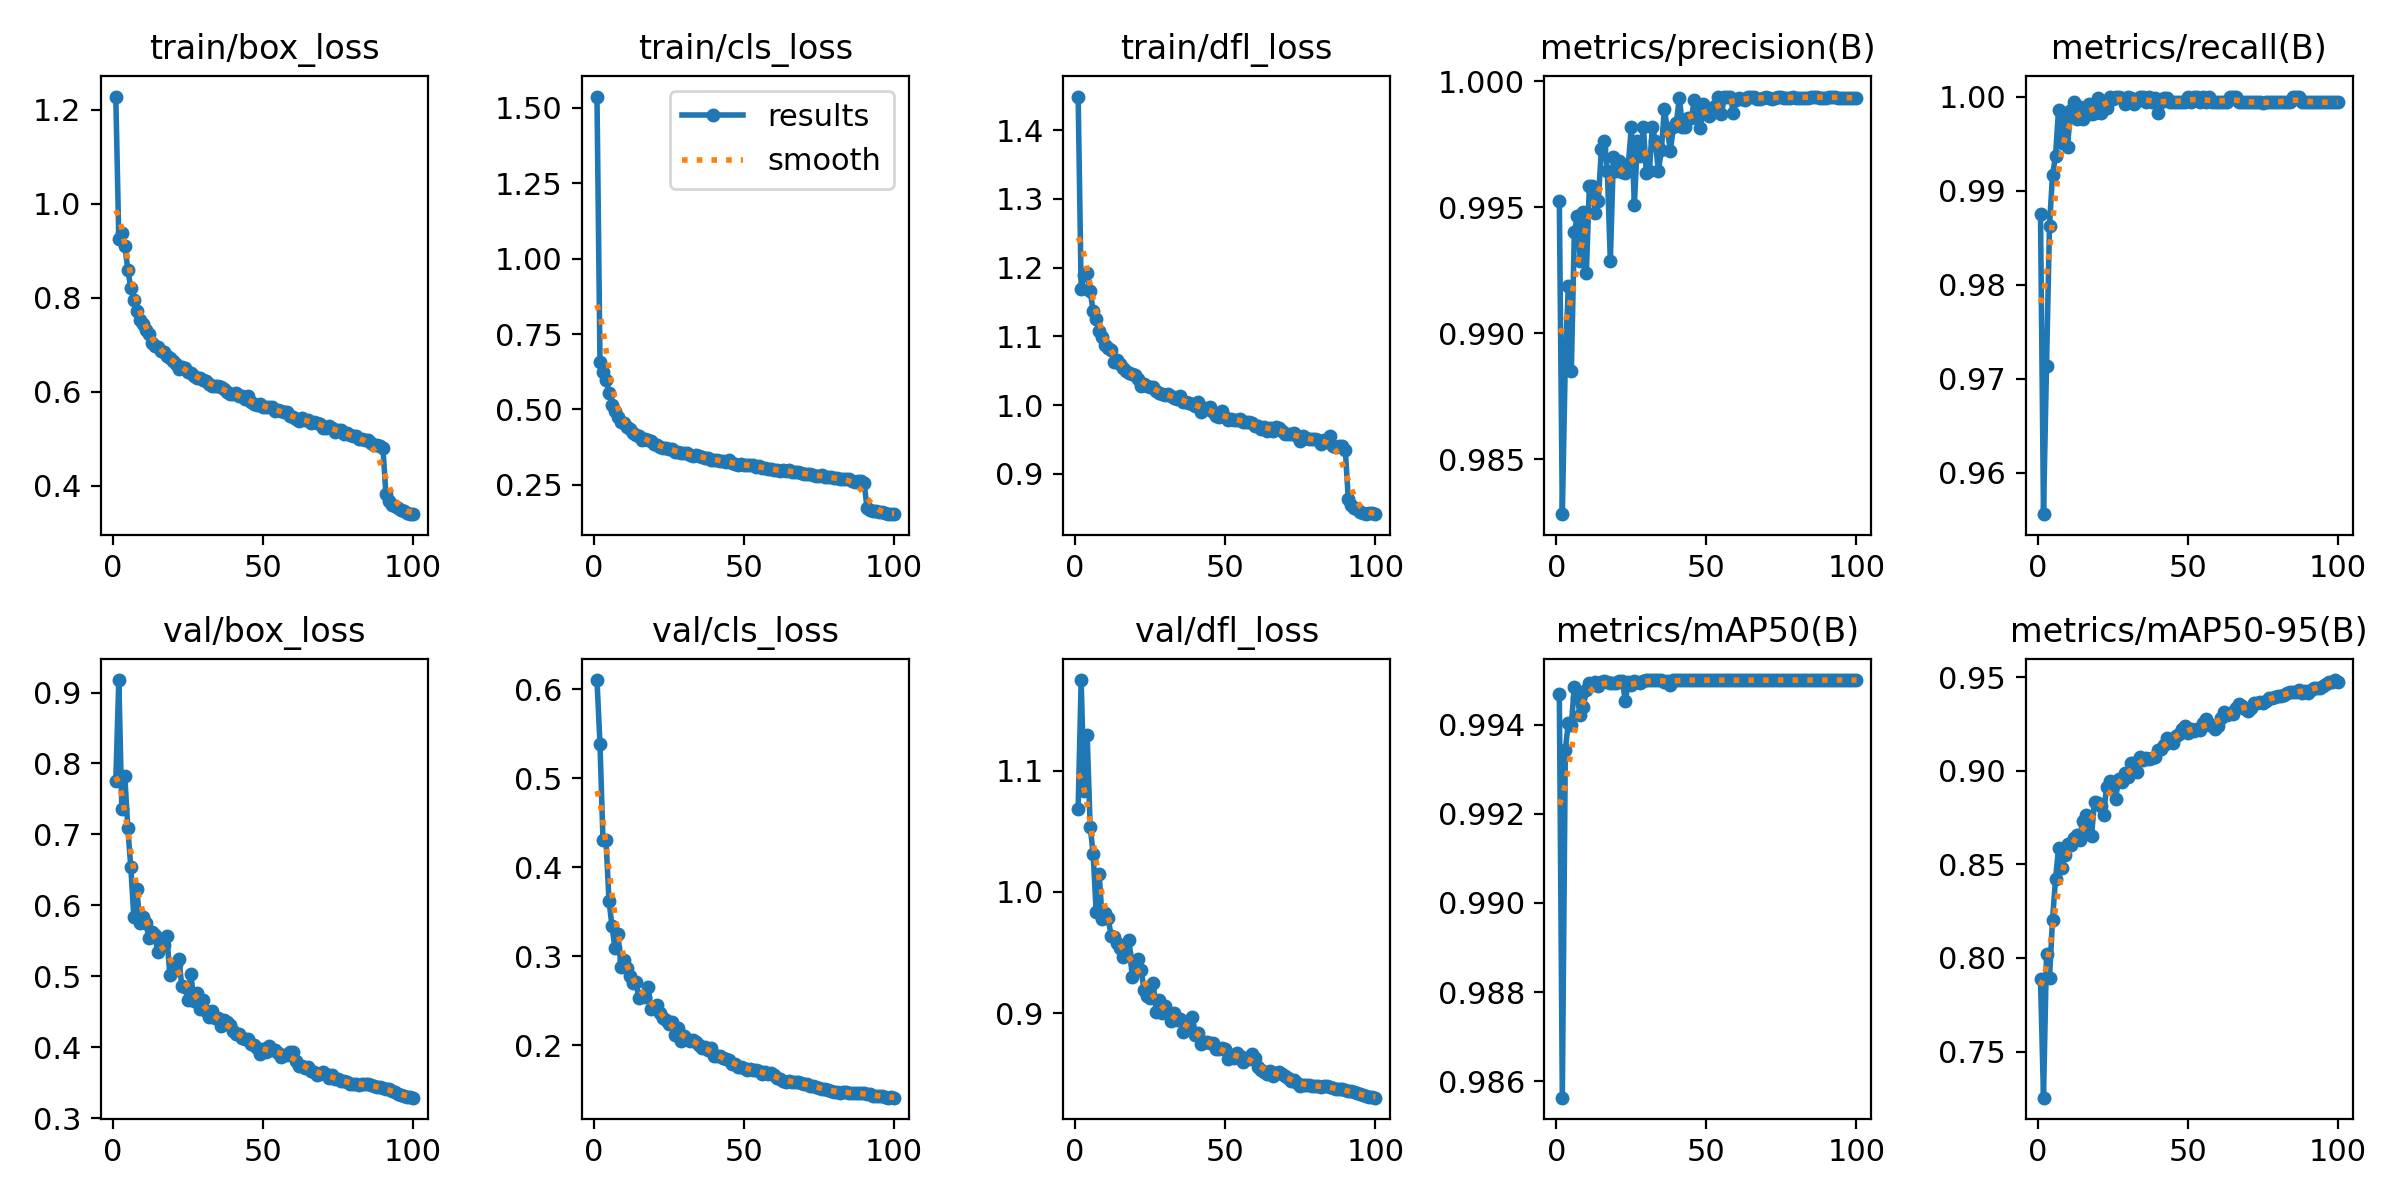
\includegraphics[width=0.8\textwidth]{images/results.png}
    \caption{Trainingsverlauf und Metriken des YOLO-Objektdetektors.}
    \label{fig:training_det}
\end{figure}

Die Wahrheitsmatrix (\emph{engl. Confusion Matrix}) der Objekterkennung (Abbildung \ref{fig:confusion_det}) verdeutlicht die Präzision bei der Lokalisierung. Sie zeigt, dass bei der Validierung 1.676 Katzengesichter korrekt erkannt wurden. Das Modell hat jedoch zwei Katzengesichter erkannt, obwohl dort keines war, und eines hat es komplett übersehen. Die Matrix belegt also dass der Detektor nahezu fehlerfrei auf den Validierungsdaten funktionierte.

\begin{figure}[H]
    \centering
    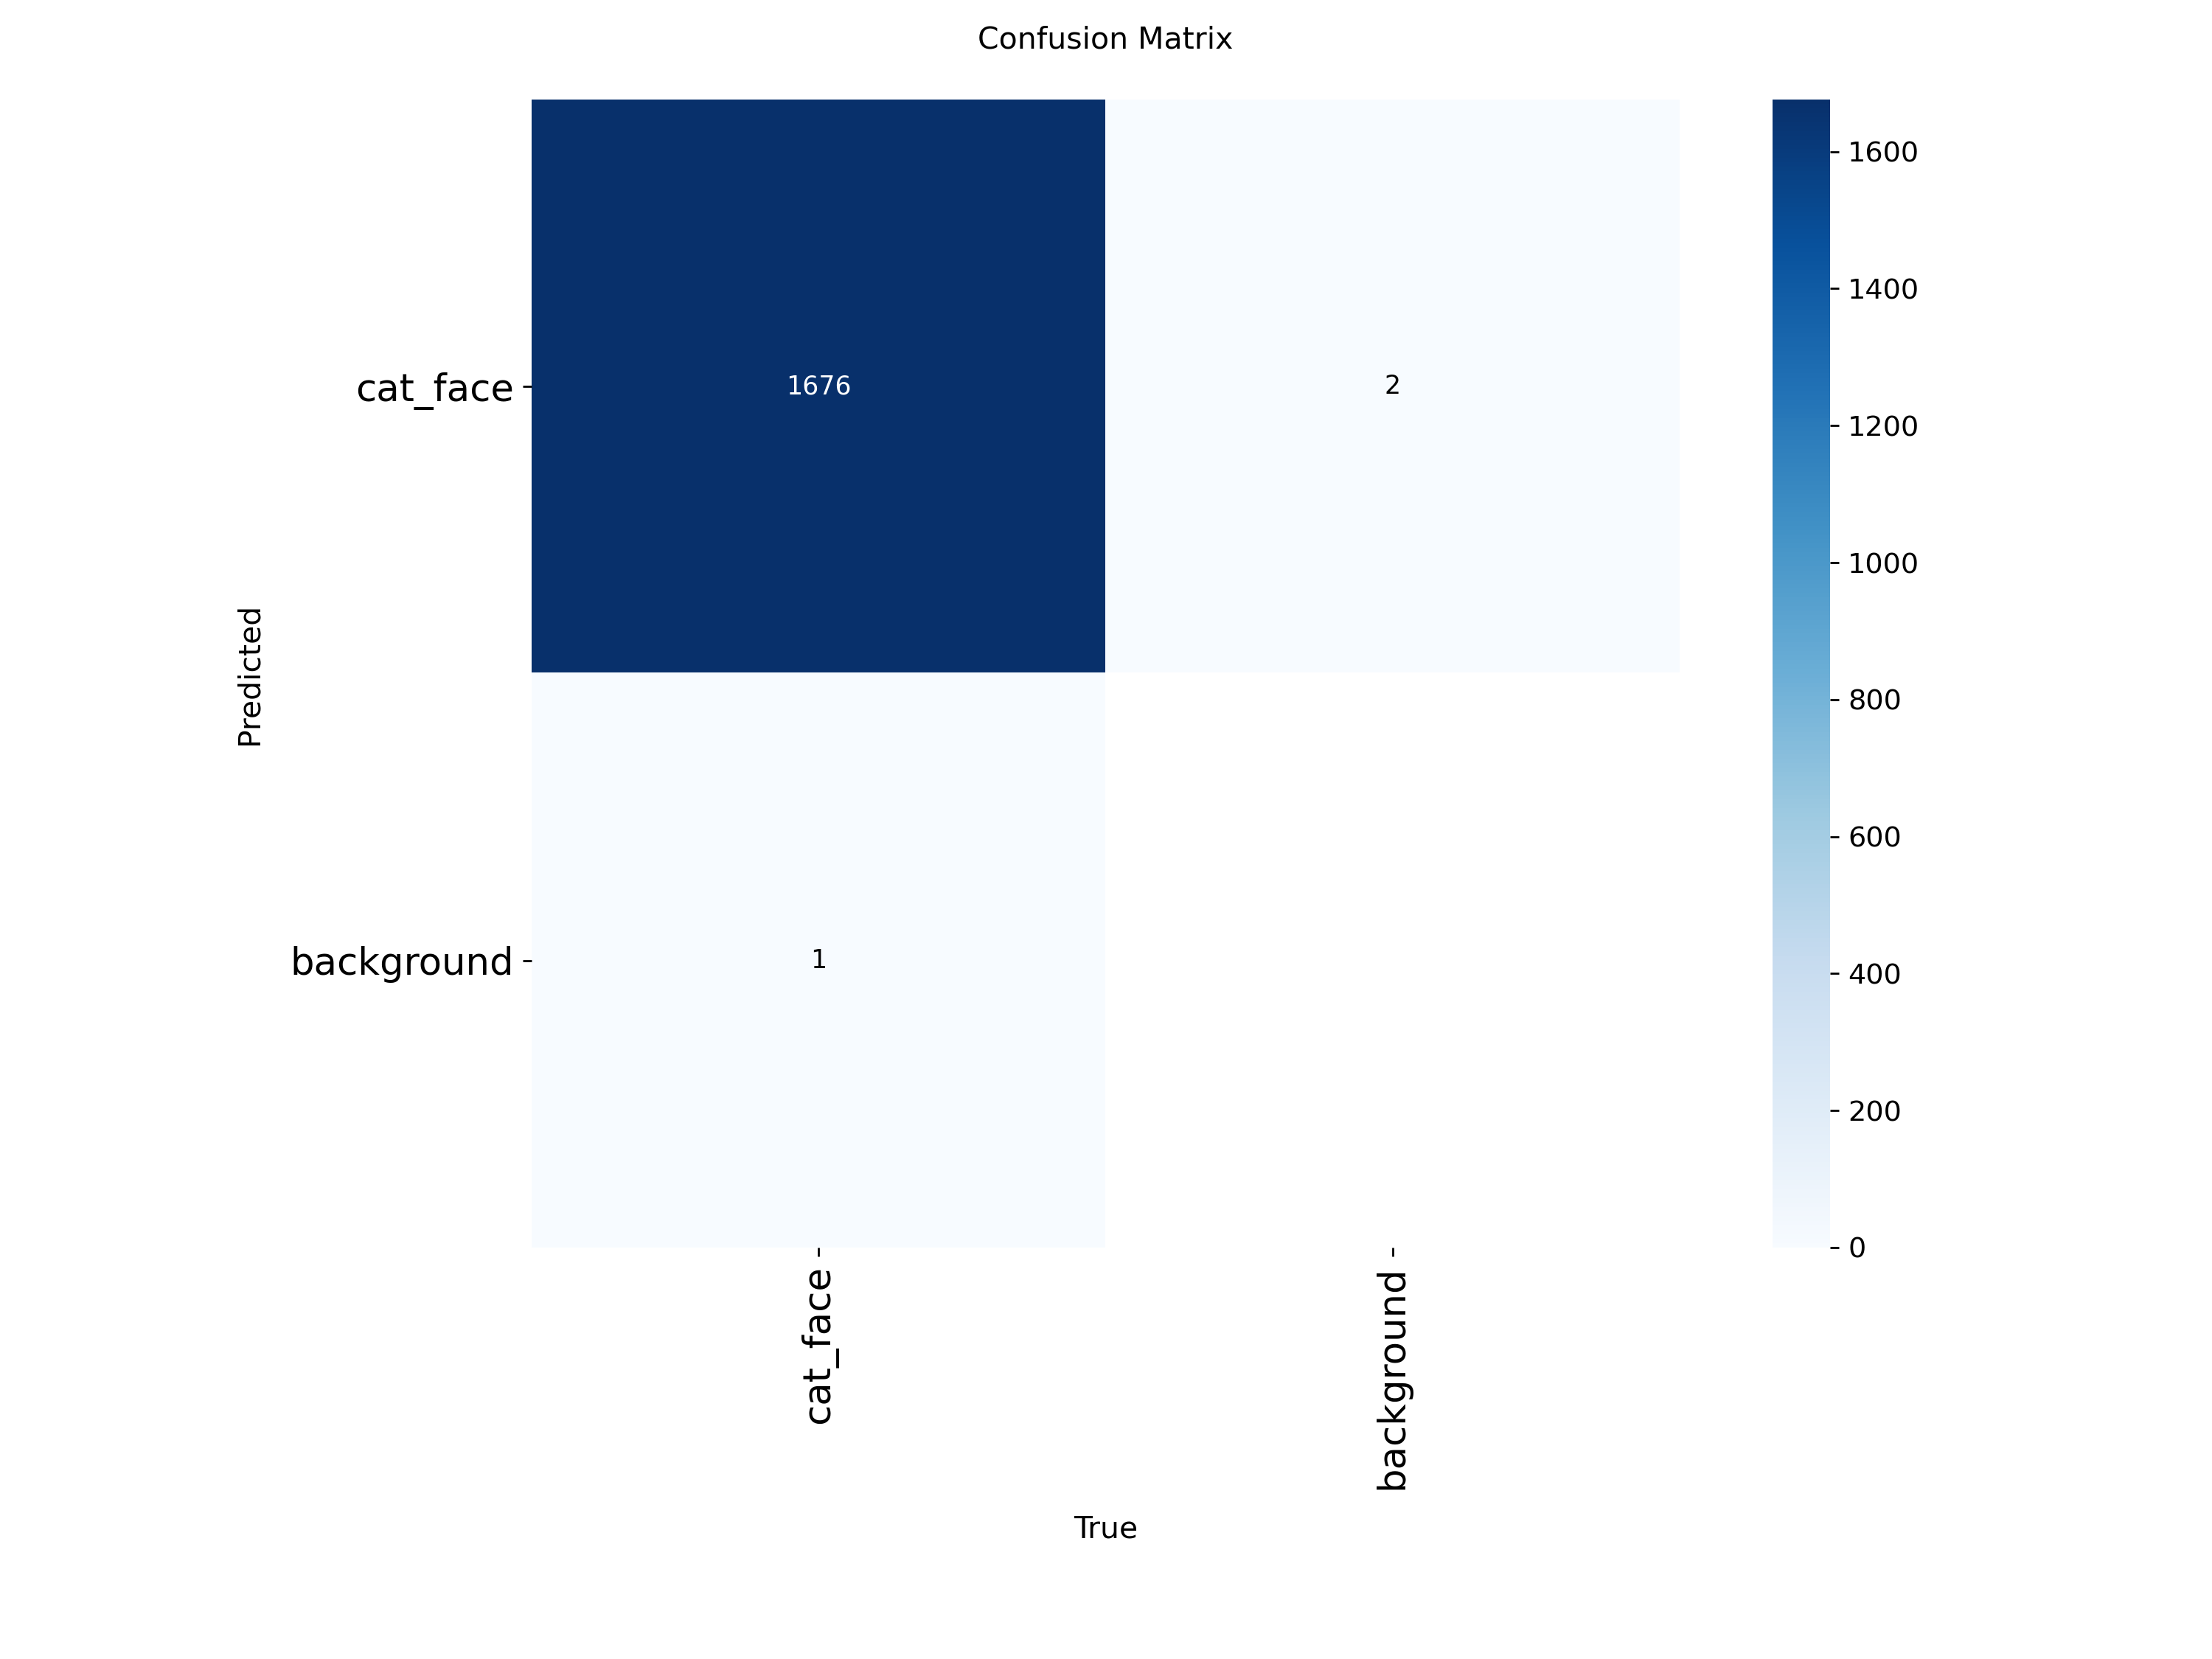
\includegraphics[width=0.6\textwidth]{images/confusion_matrix.png}
    \caption{Wahrheitsmatrix (Detektor).}
    \label{fig:confusion_det}
\end{figure}

Eine wichtige Metrik, welche auch auf den Validierungsdaten beruht, ist die Präzision-Trefferquote-Kurve (\emph{engl. Precision-Recall-Curve}), sie gibt das Verhältnis zwischen richtig erkannten Objekten und Fehlalarmen an wie sicher  das Modell ist \cite{everingham2010pascal, lin2014coco}. In diesem Fall zeigt der Verlauf, dass das Modell extrem sicher ist und nicht raten muss, wenn es ein Katzengesicht sieht.

\begin{figure}[H]
    \centering
    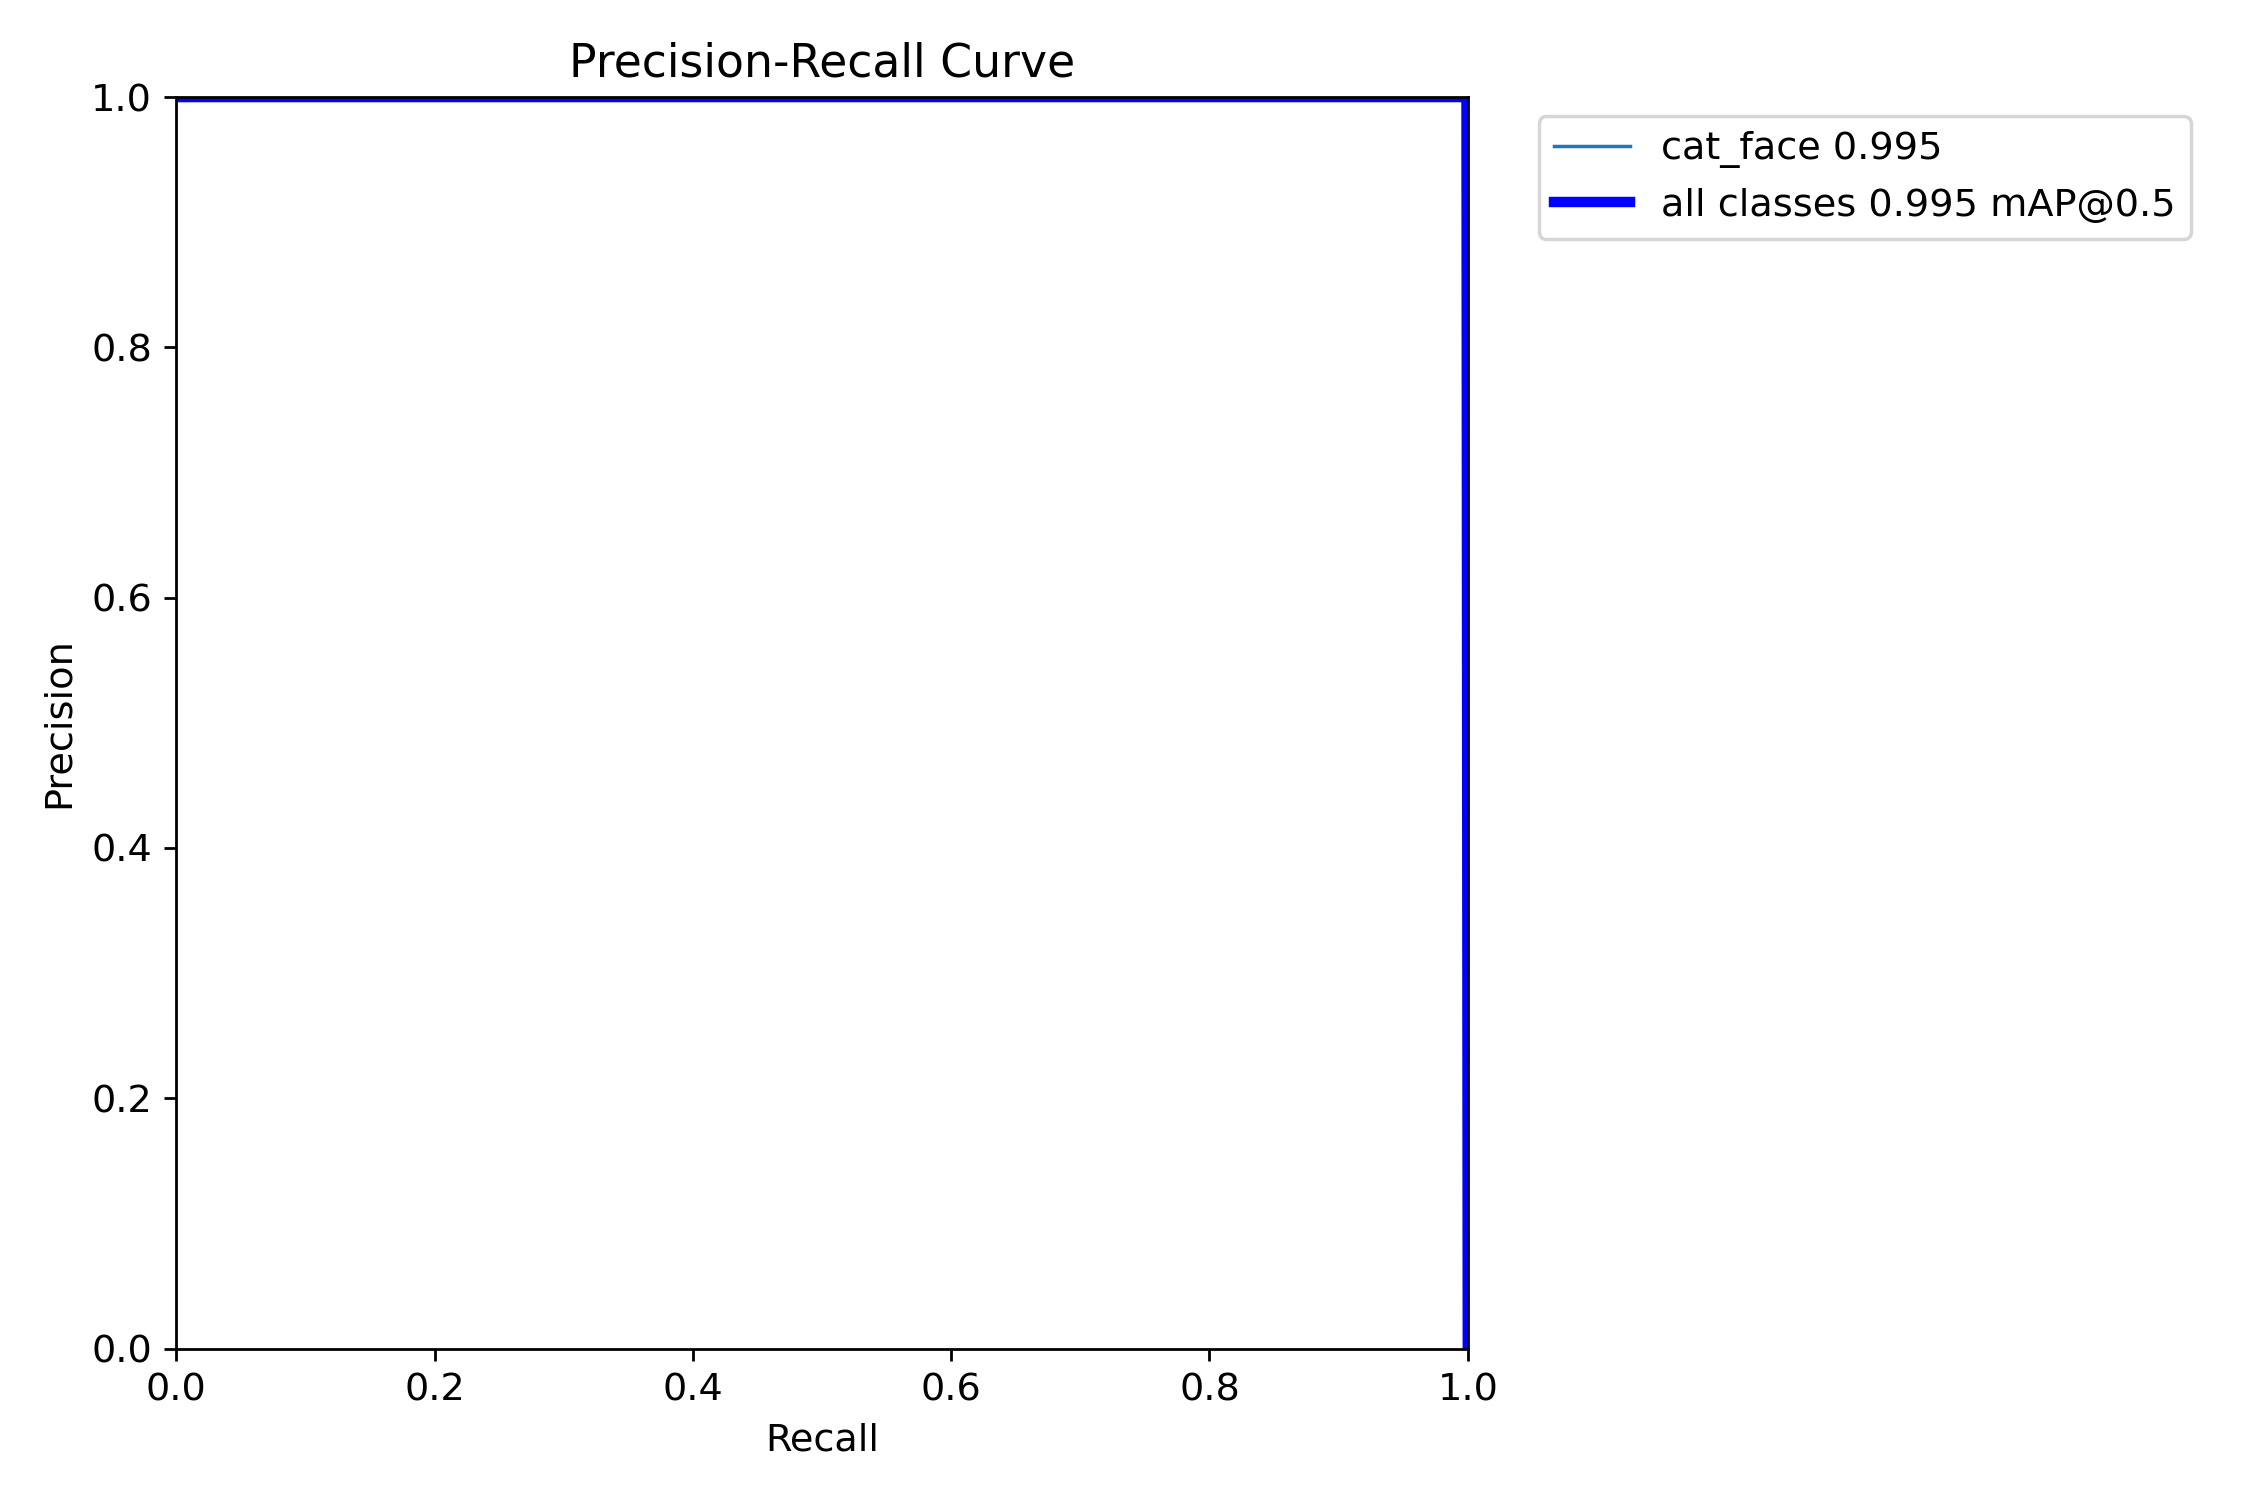
\includegraphics[width=0.6\textwidth]{images/BoxPR_curve.png}
    \caption{Präzision-Trefferquote-Kurve (\emph{engl. Precision-Recall-Curve}).}
    \label{fig:pr_curve_det}
\end{figure}

Die F1-Maß-Kurve (Abbildung \ref{fig:f1_curve_det}) zeigt wie sich die Leistung des Modells bei Änderung des Konfidenzschwellenwerts \cite{ultralytics_confidence} verändert. Dadurch können wir den optimalen Schwellenwert für den realen Betrieb des Modells ermitteln. Da die Kurve bis $\approx 0,85$ flach bleibt, d.h. hier wird keine Katze übersehen, fällt sie $> 0{,}85$ stark ab. Das zeigt, dass ab diesem Schwellenwert auch reale Katzen leicht übersehen werden. In der Praxis zeigt sich, dass bei einem Konfidenzschwellwert von $\approx 0,75$ ein gutes Verhältnis zwischen „Katze wird nicht erkannt“ und „es wird eine Katze erkannt, wo sich keine befindet“ entsteht. Im Betrieb wird der Detektor dennoch mit einem niedrigen Schwellenwert von 0,1 ausgeführt, da ByteTrack auch Erkennungen mit niedrigem Konfidenzwert für die Zuordnung verwendet \cite{zhang2022bytetrack}.

\begin{figure}[H]
    \centering
    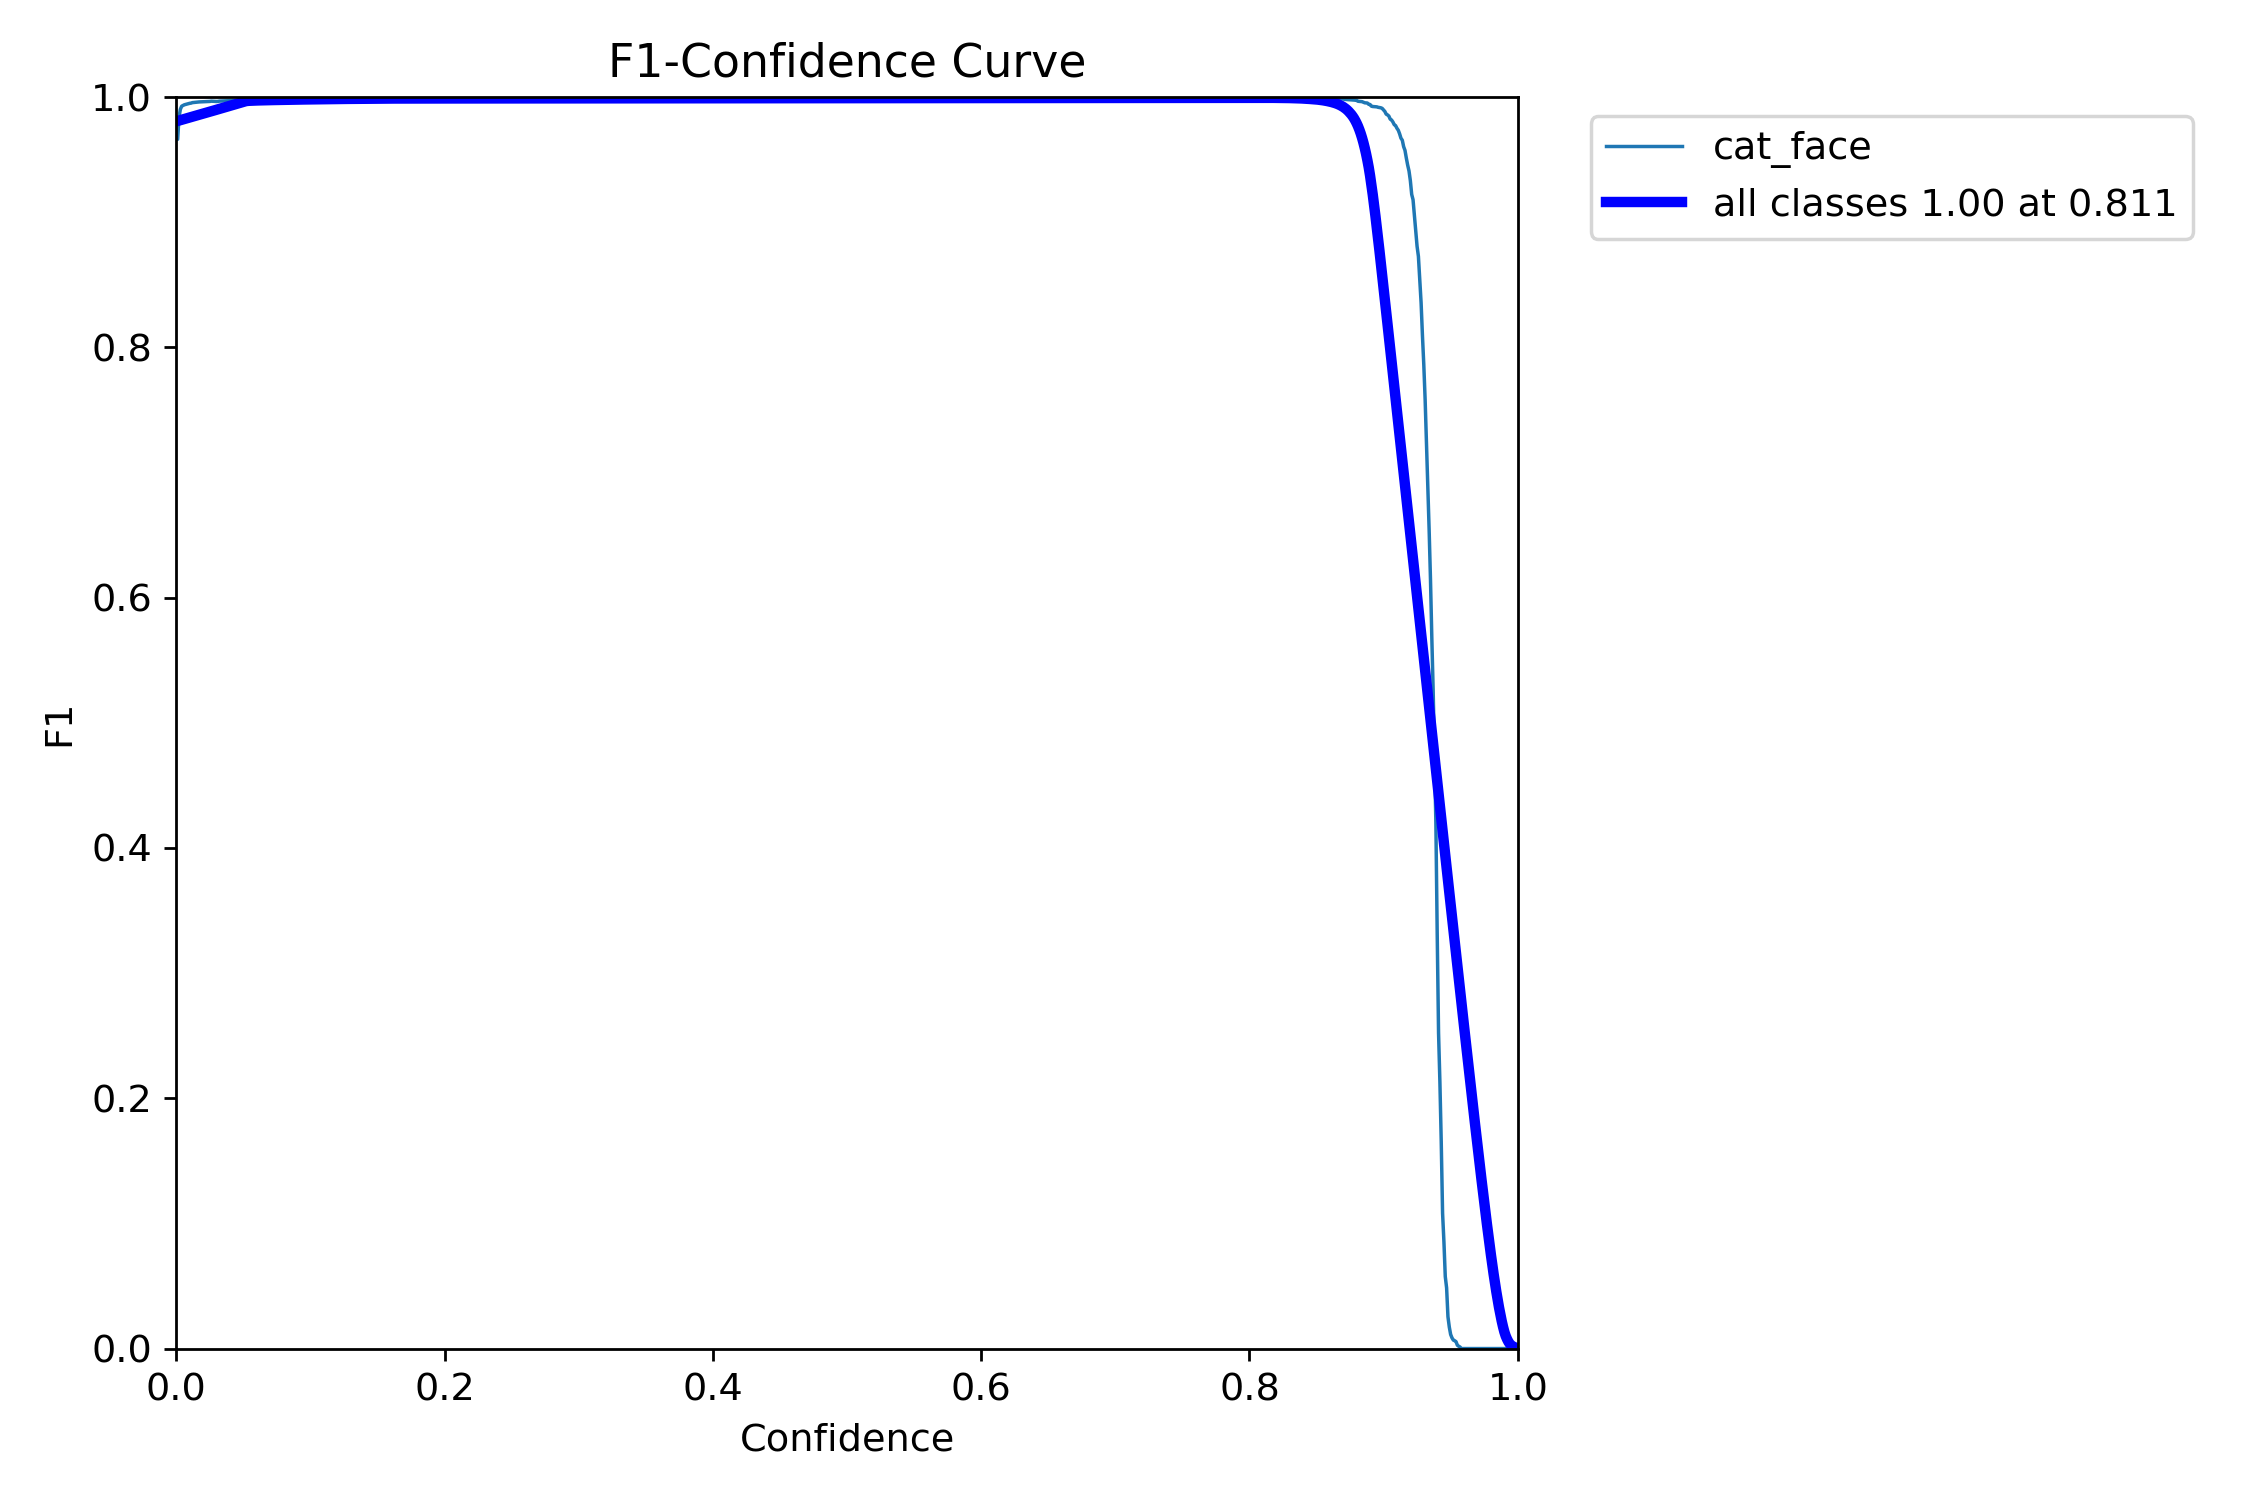
\includegraphics[width=0.6\textwidth]{images/BoxF1_curve.png}
    \caption{F1-Maß-Kurve.}
    \label{fig:f1_curve_det}
\end{figure}

Die Abbildung \ref{fig:val_pred_det} liefert einen Eindruck auf die Erkennungsleistung des Modells, wenn man es auf die Validierungsdaten ansetzt.

\begin{figure}[H]
    \centering
    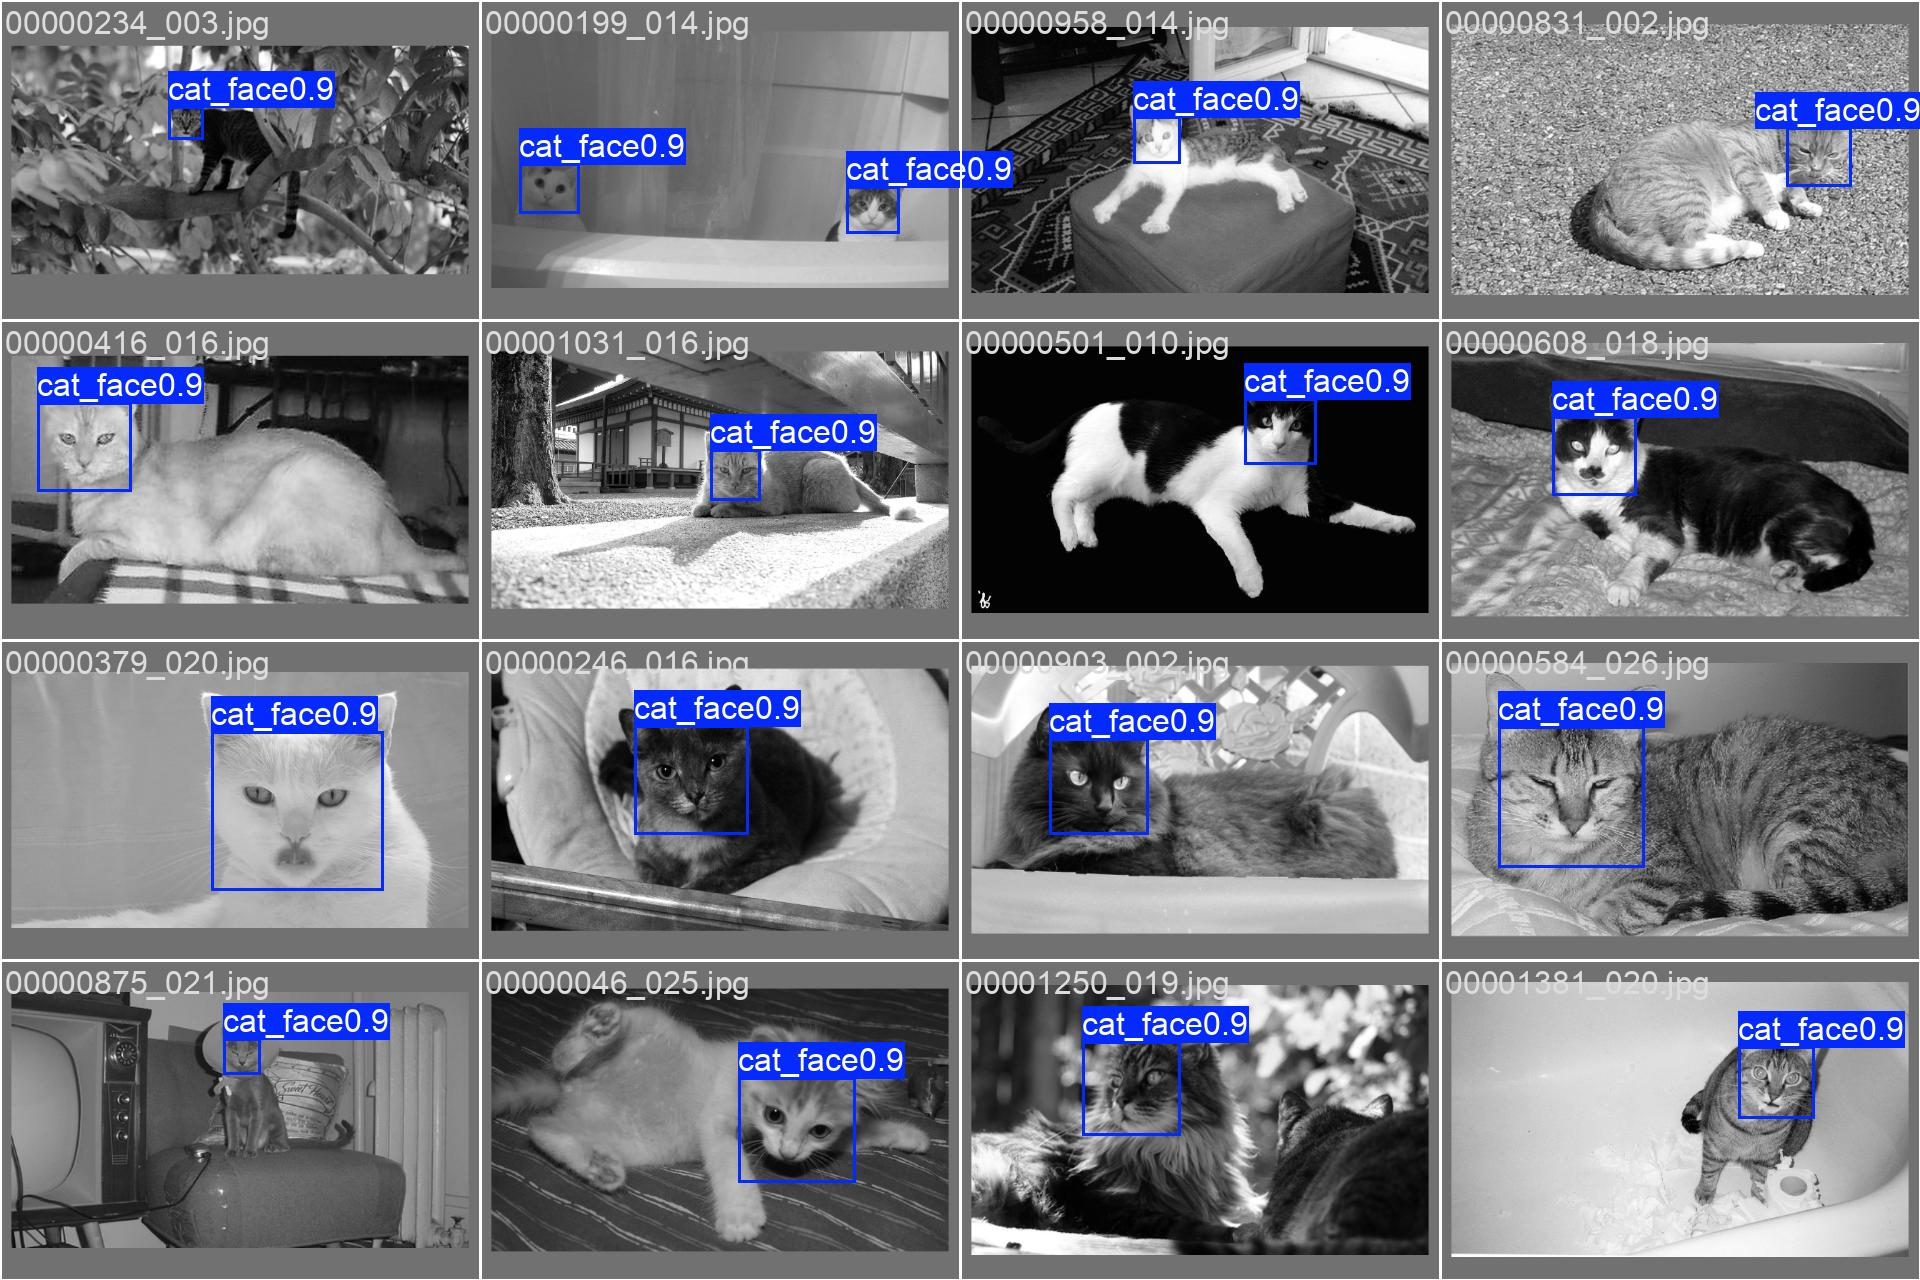
\includegraphics[width=0.8\textwidth]{images/val_batch0_pred.jpg}
    \caption{Vorhersagen des Detektors auf dem Validierungsdatensatz.}
    \label{fig:val_pred_det}
\end{figure}

\subsection{Leistung der Bildsegmentierung}
Die folgenden Trainingsmetriken des Beute-Segmentierungsmodells zeigen, dass das Modell seine Aufgabe erfolgreich gelernt hat.
Beim betrachten der Verlustfunktionen wird ersichtlich, dass das Modell über die Epochen weniger Fehler sowohl bei Training als auch Validierung macht, daraus können wir schließen, dass das Segmentierungsmodell lernt ohne sich dabei zu viel auf den Trainingsdatensatz anpasst.

\begin{figure}[H]
    \centering
    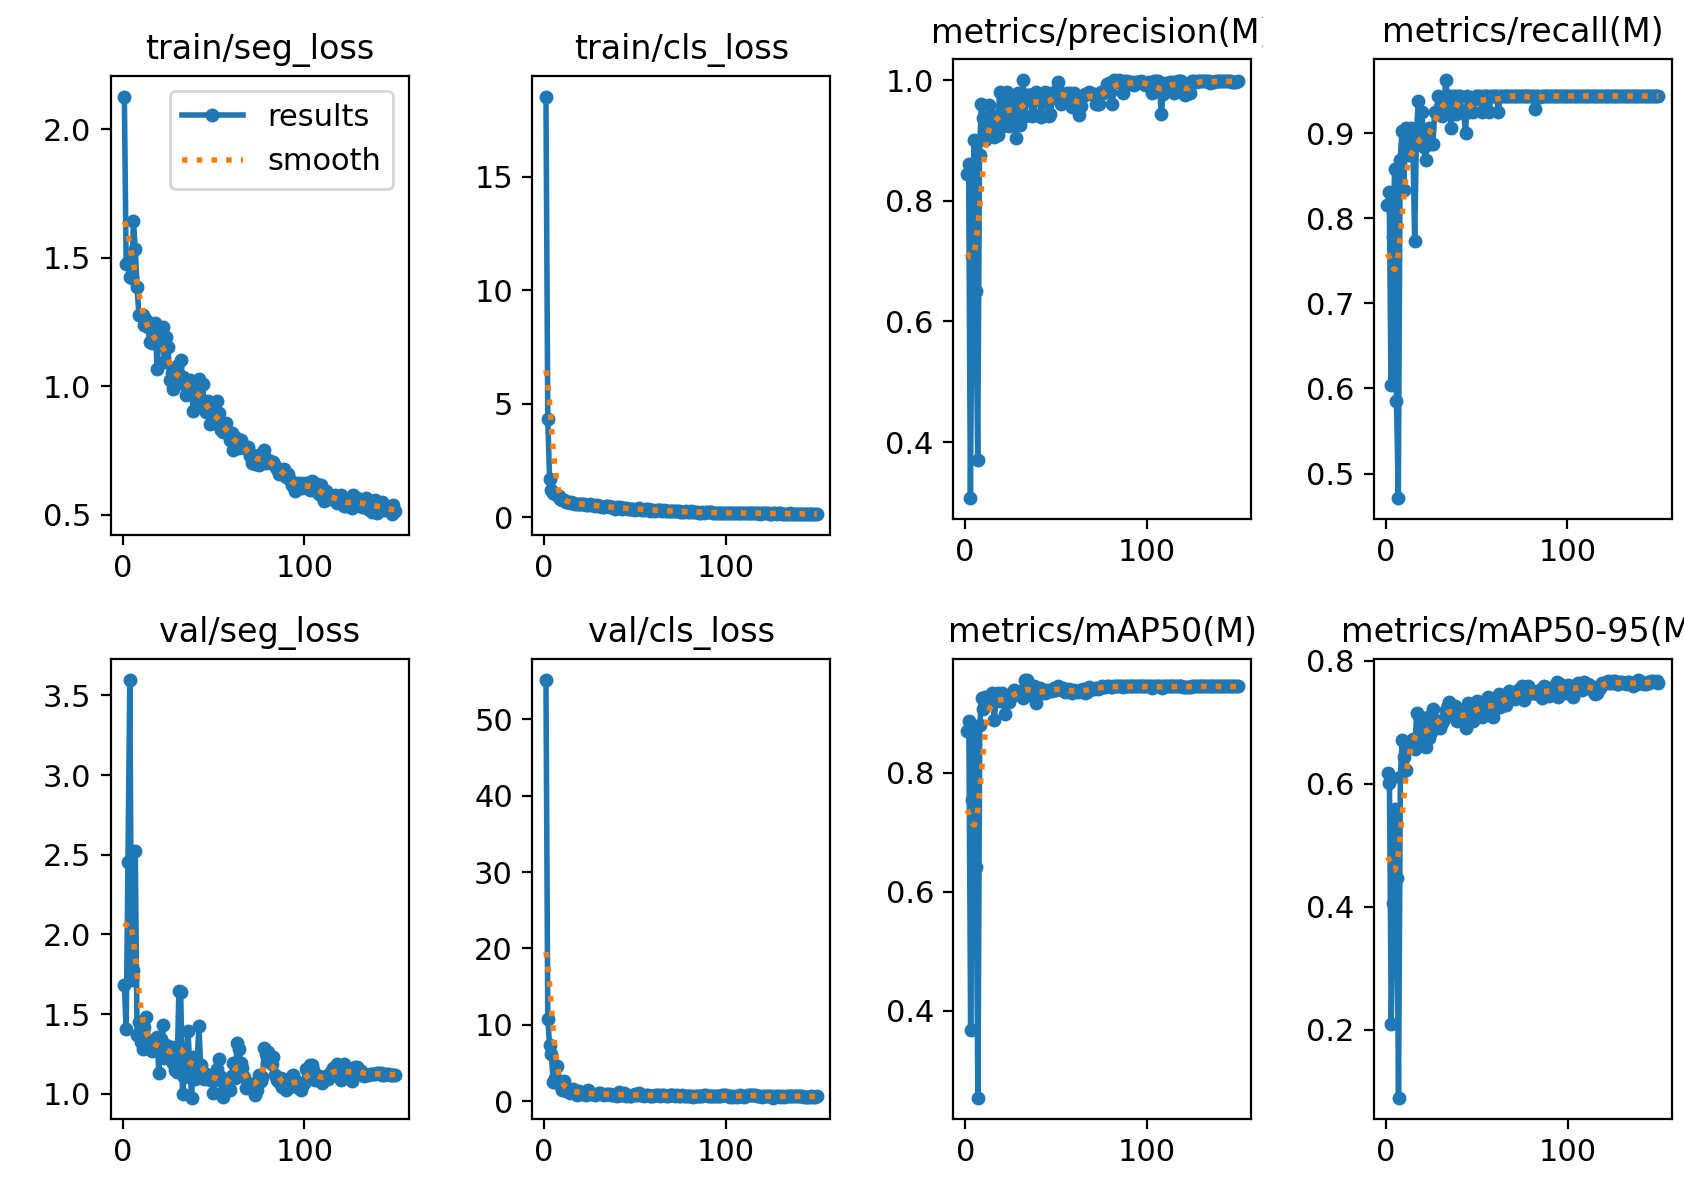
\includegraphics[width=0.8\textwidth]{images/seg_results.png}
    \caption{Trainingsverlauf und Metriken des YOLO-Segmentierungsmodells.}
    \label{fig:training_cls}
\end{figure}

Die Präzision-Trefferquote-Kurve der Segmentierungsmasken (Abbildung \ref{fig:pr_curve_seg}) zeigt, dass das Modell bis zu einer Trefferquote von etwa 94\,\% keine einzige Fehlerkennung liefert. Auf dem Validierungsdatensatz erreicht es eine mAP50 von 0,945.

\begin{figure}[H]
    \centering
    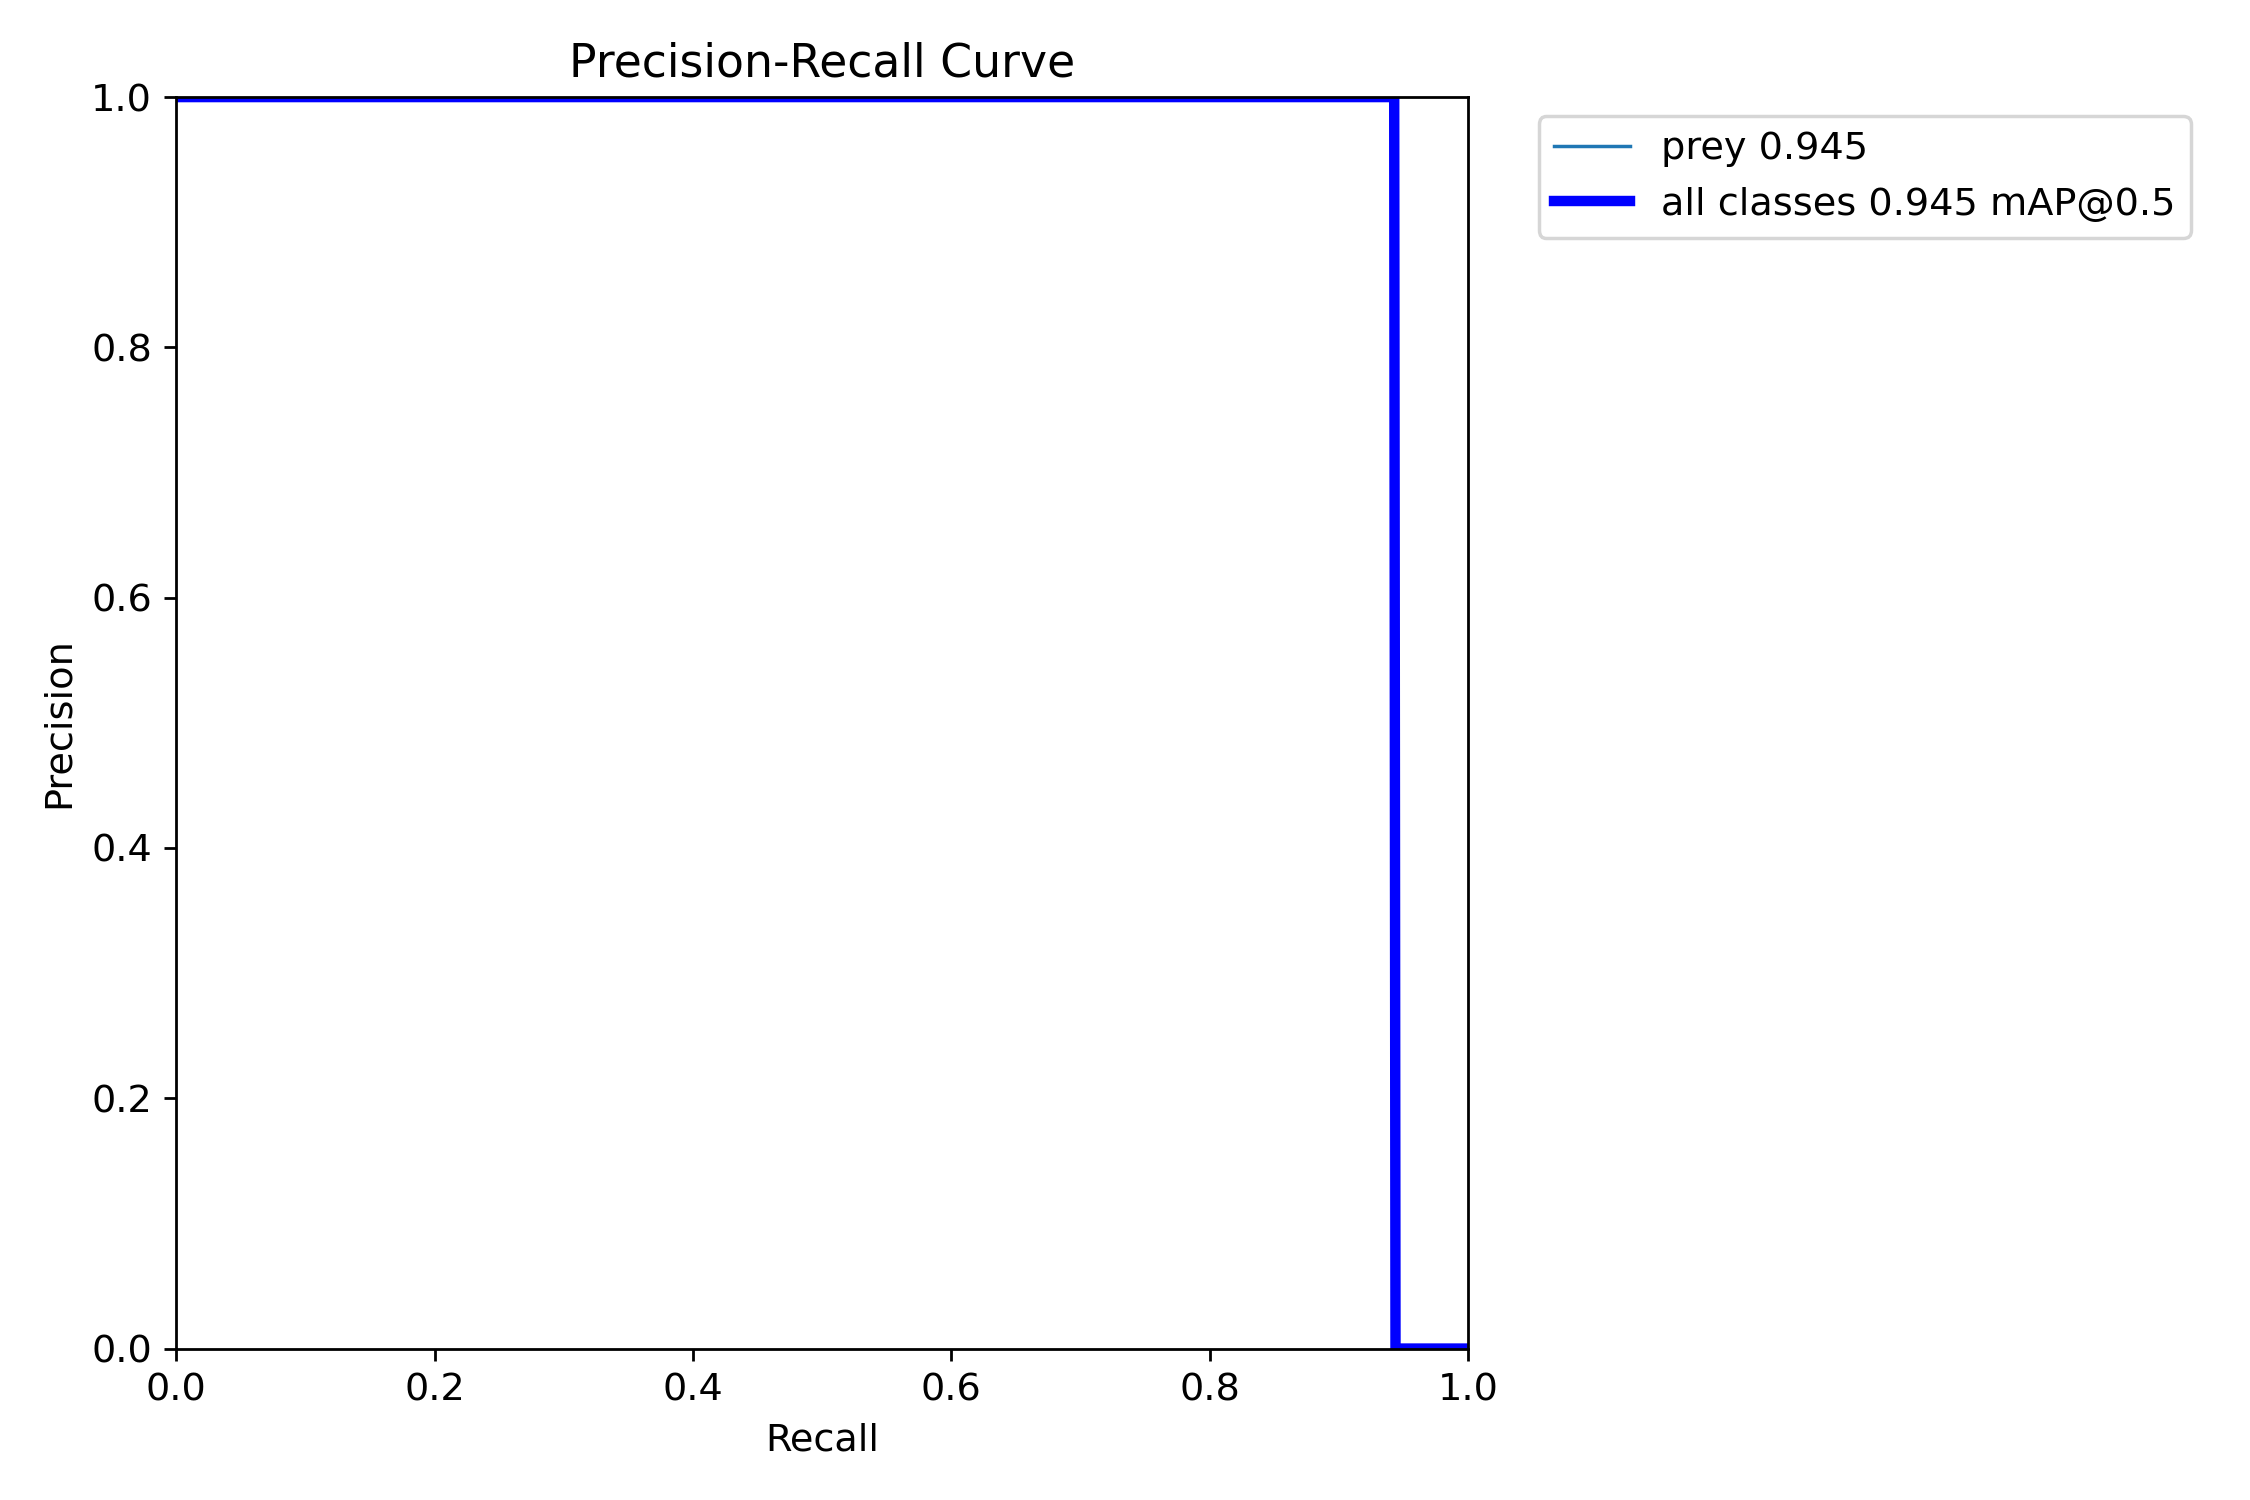
\includegraphics[width=0.6\textwidth]{images/seg_pr_curve.png}
    \caption{Präzision-Trefferquote-Kurve der Segmentierungsmasken.}
    \label{fig:pr_curve_seg}
\end{figure}

Die F1-Maß-Kurve (Abbildung \ref{fig:f1_curve_seg}) erreicht ihr Maximum von 0,97 bei einem Konfidenzschwellenwert von 0,728. Zwischen etwa 0,1 und 0,85 bleibt sie nahezu konstant, das Modell reagiert in diesem Bereich also kaum empfindlich auf die Wahl des Schwellenwerts.

\begin{figure}[H]
    \centering
    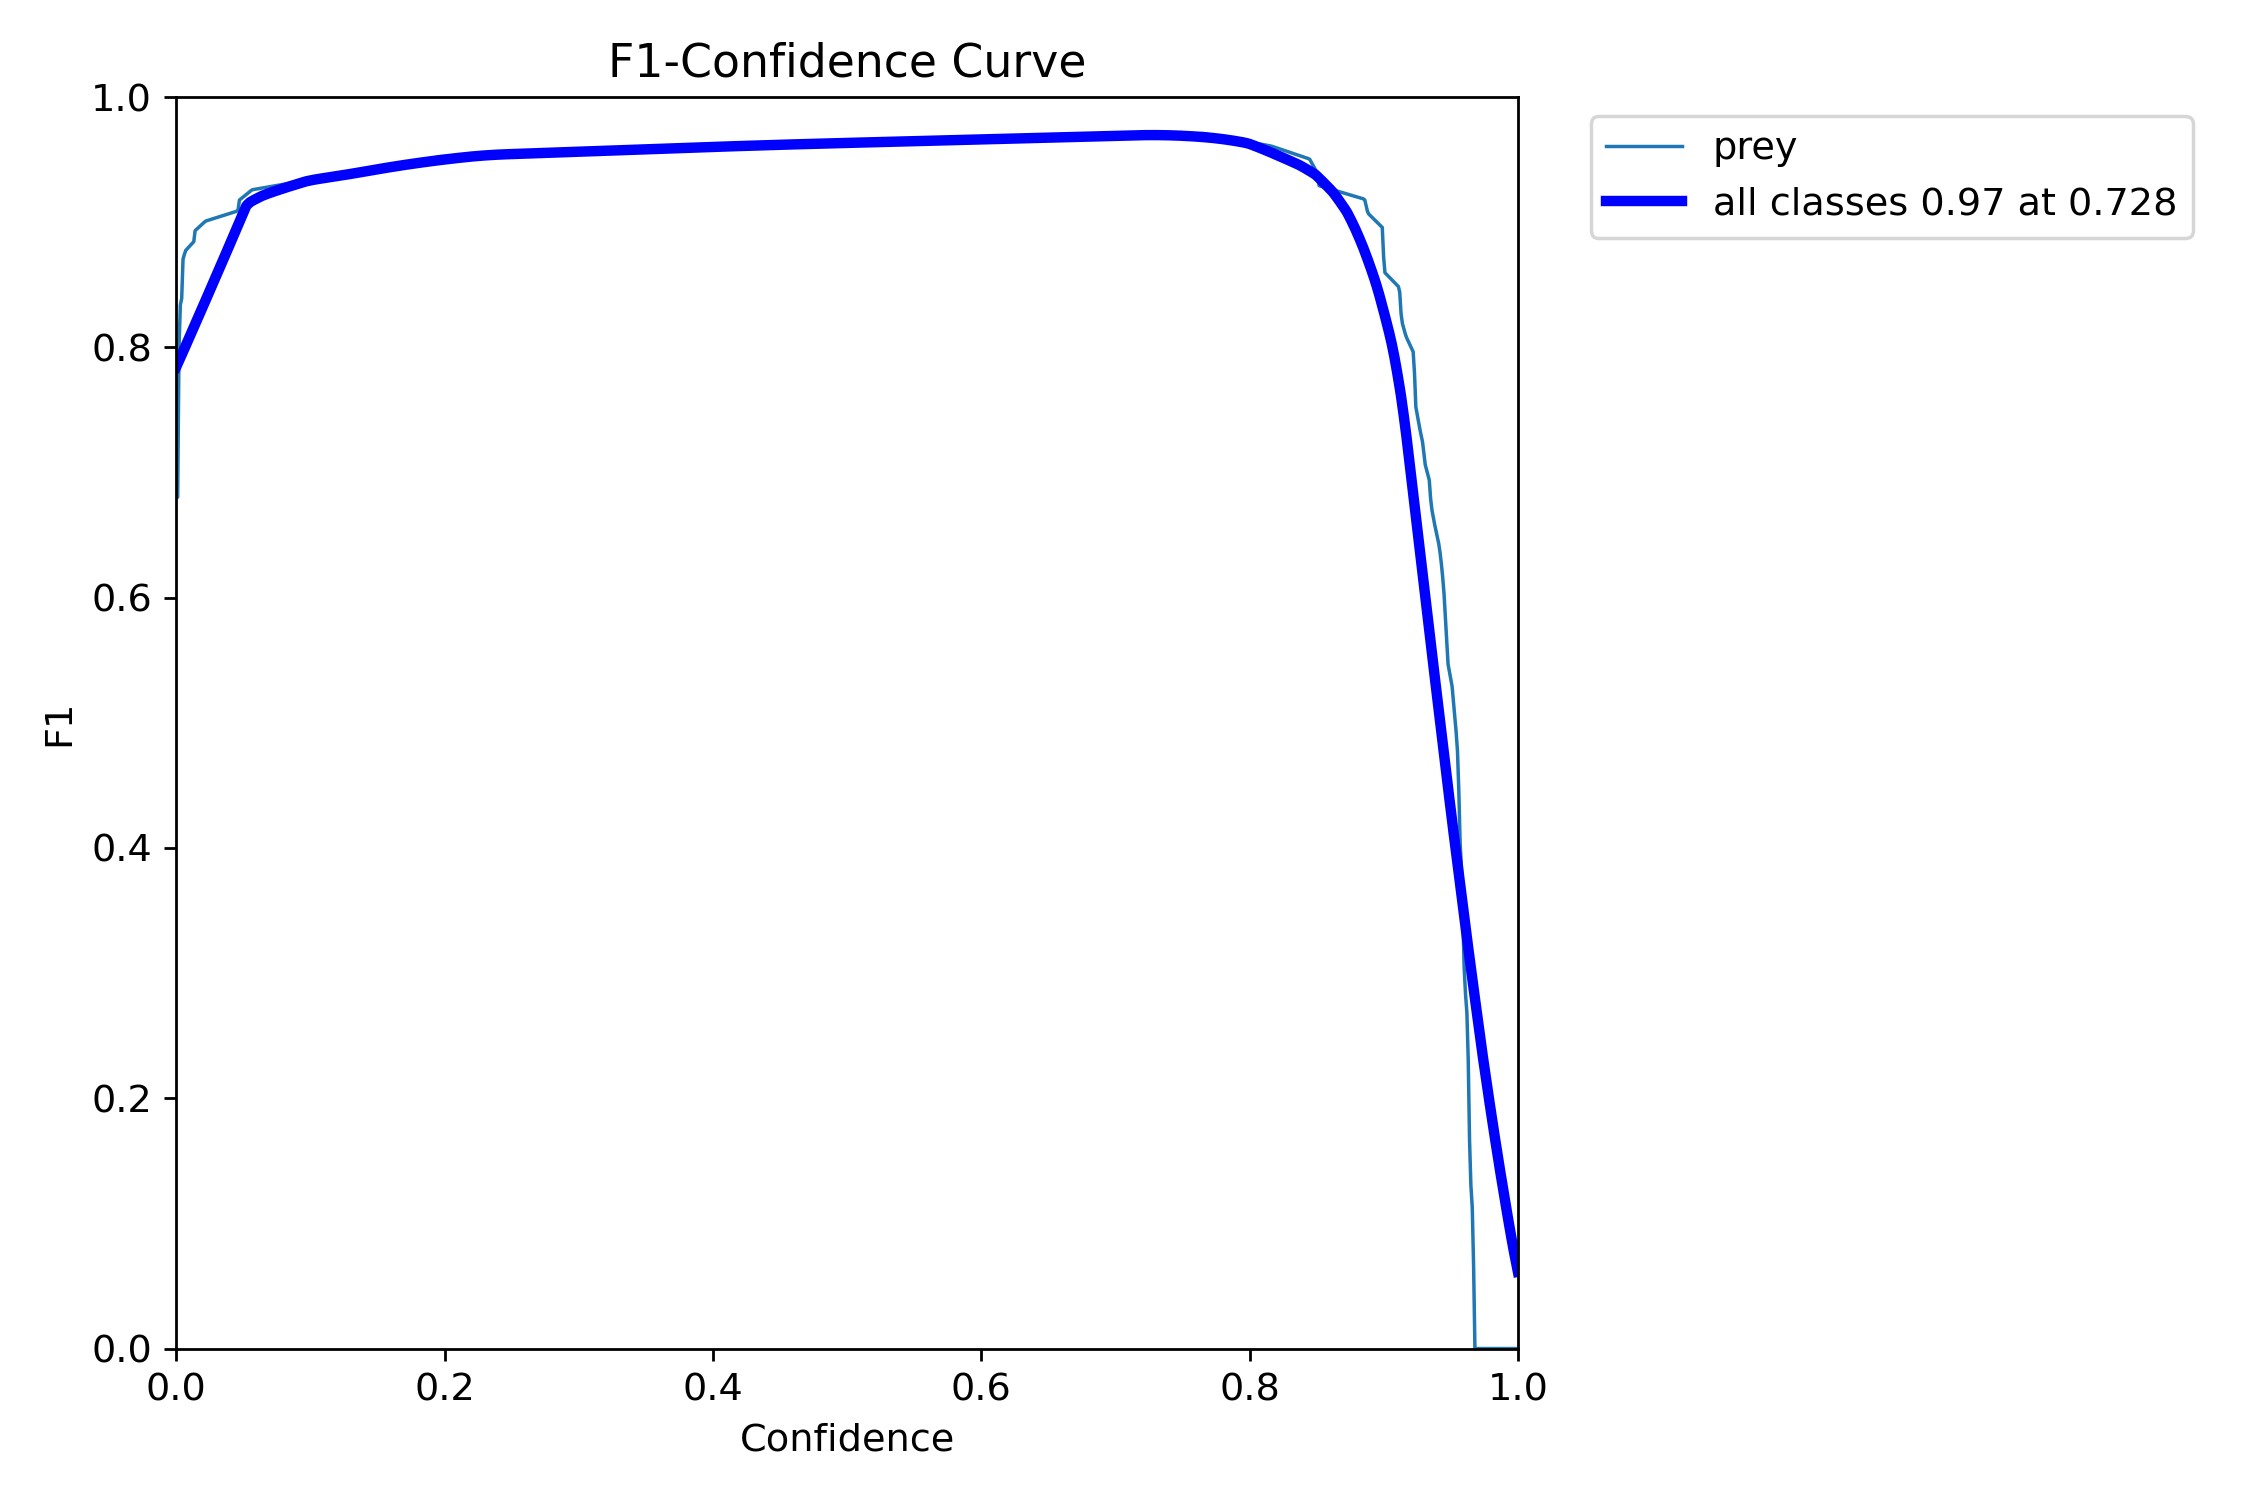
\includegraphics[width=0.6\textwidth]{images/seg_f1_curve.png}
    \caption{F1-Maß-Kurve des Segmentierungsmodells.}
    \label{fig:f1_curve_seg}
\end{figure}

Mithilfe der Abbildung \ref{fig:val_pred_cls} lässt sich gut erkennen, wie gut das Modell mit unbekannten Daten umgeht.

\begin{figure}[H]
    \centering
    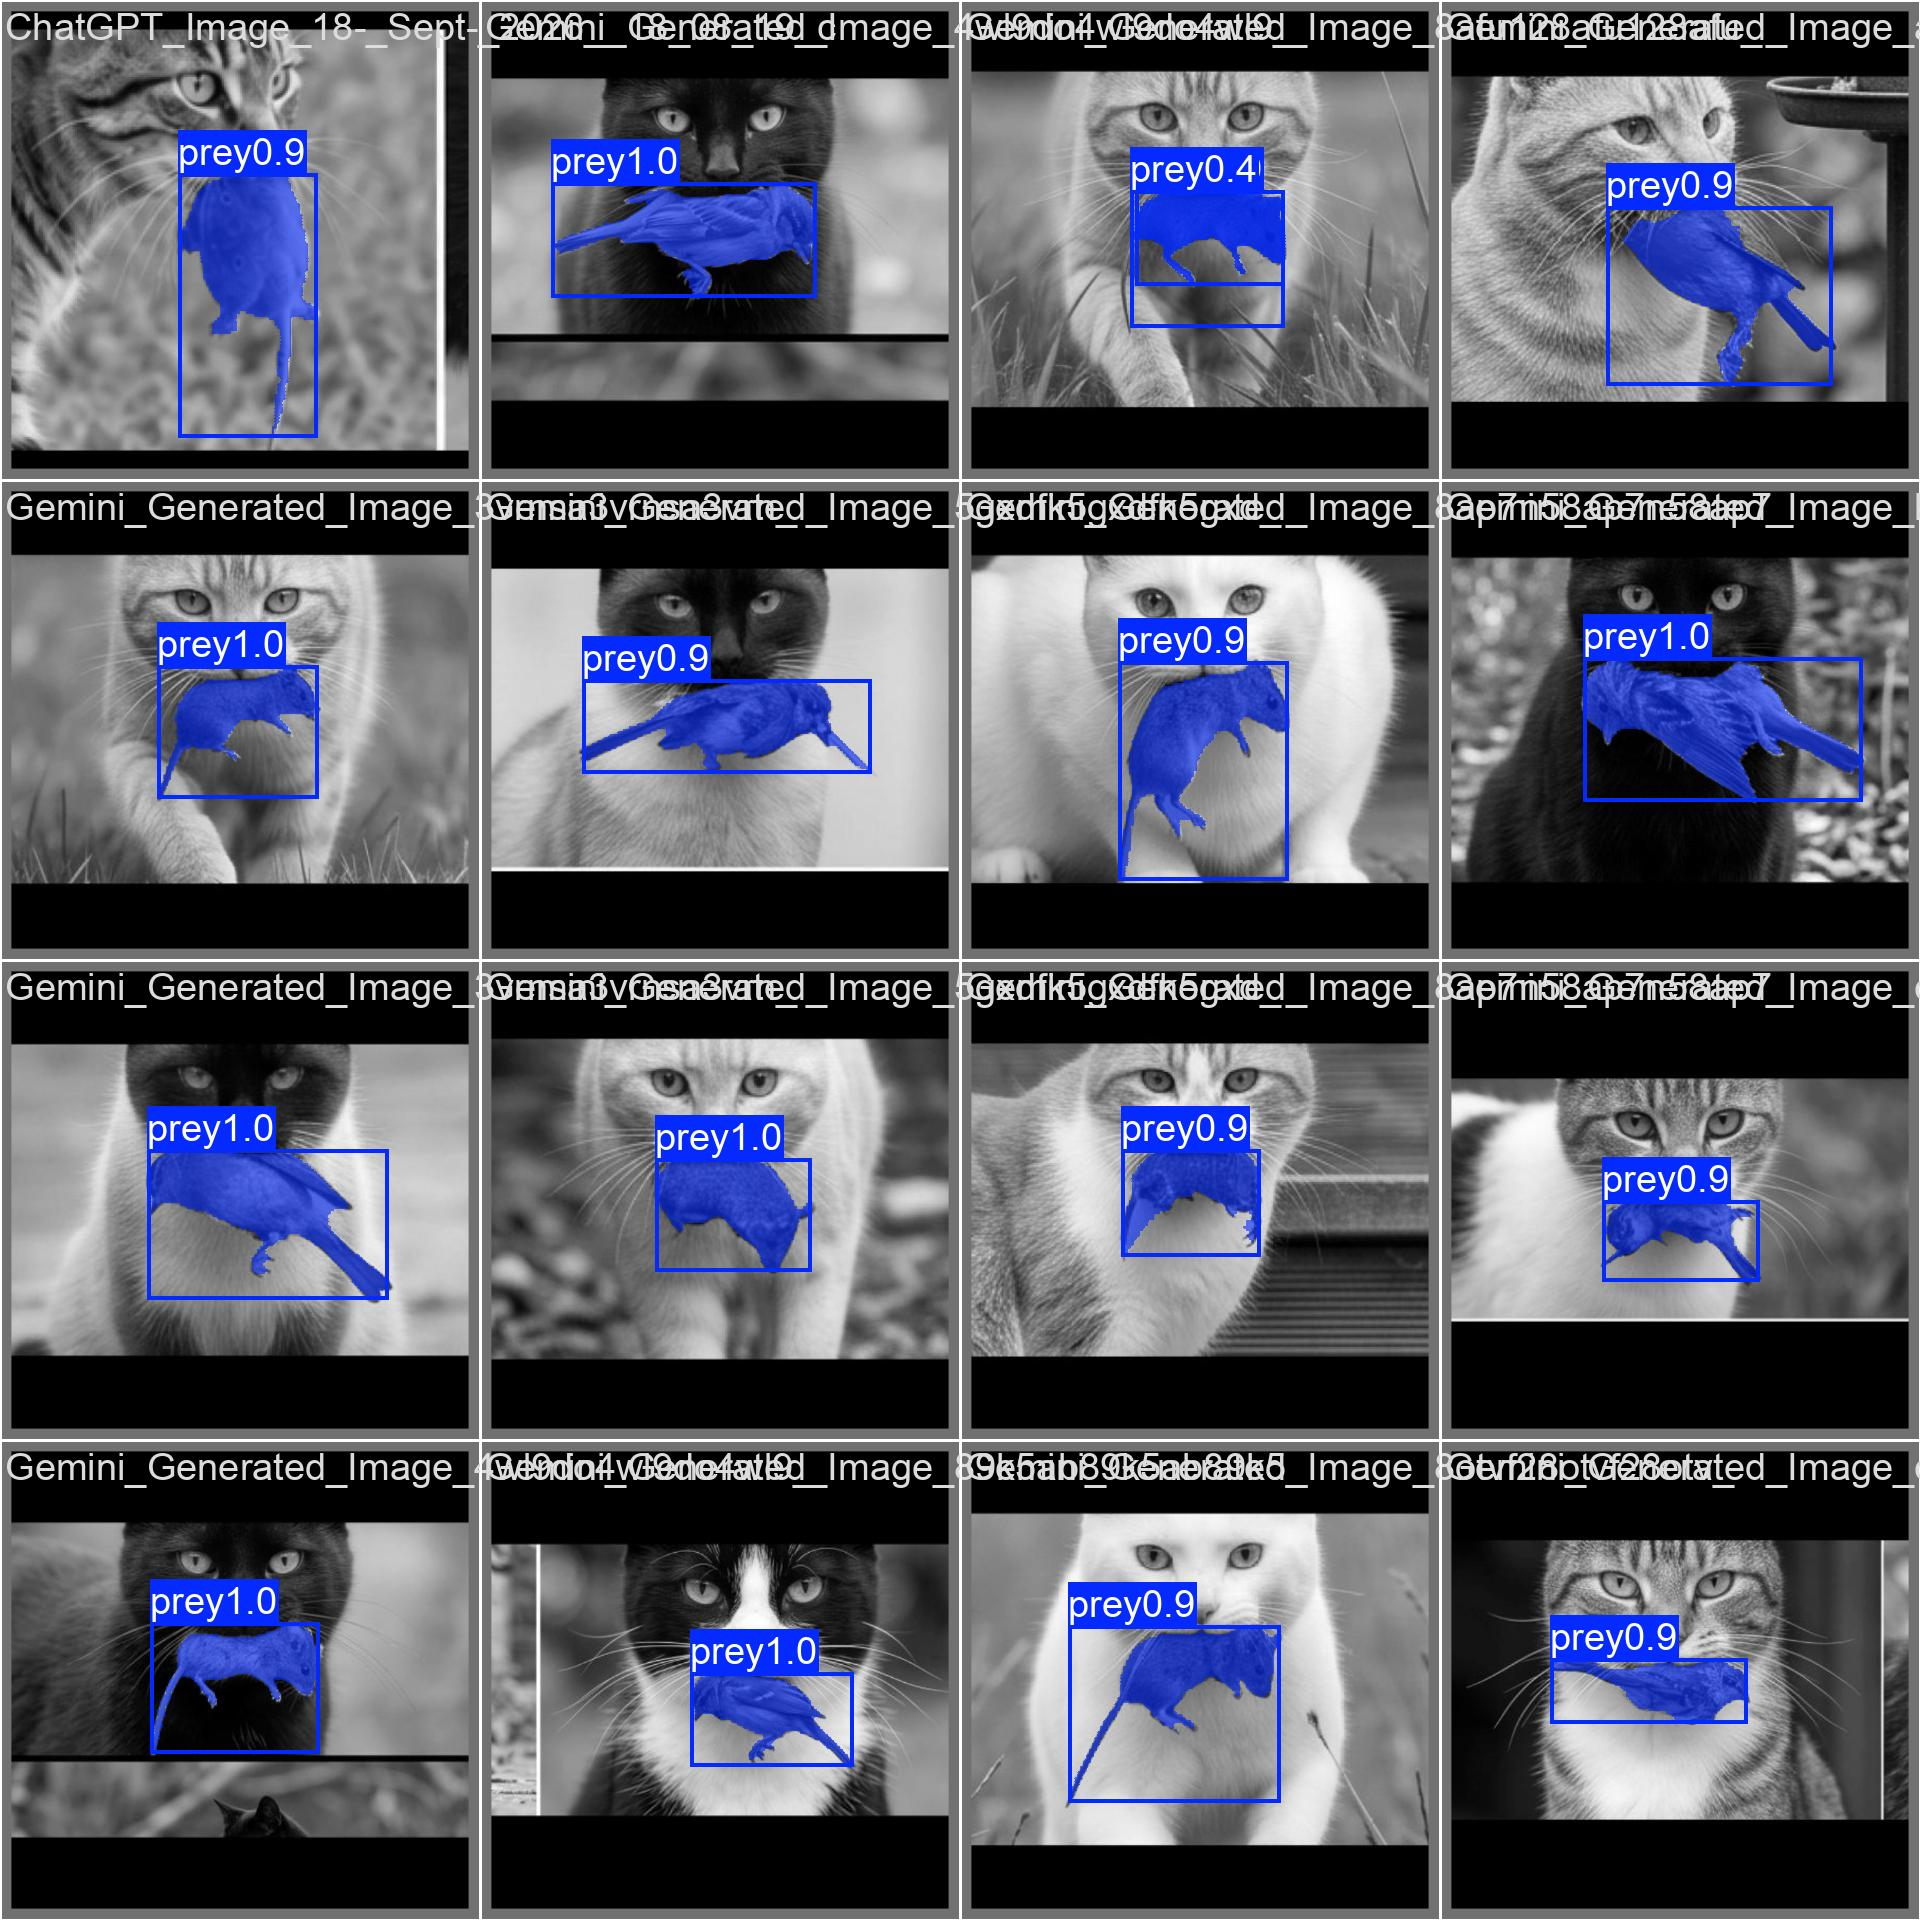
\includegraphics[width=0.8\textwidth]{images/seg_val_pred.jpg}
    \caption{Beispielhafte Vorhersagen des Segmentierungsmodells auf dem Validierungsdatensatz.}
    \label{fig:val_pred_cls}
\end{figure}

Rein auf dem Papier würden diese Modelle fast fehlerfreie Aussagen treffen. Die entscheidende Frage ist jedoch, wie verhält sich das System im Praxiseinsatz und welche Vorteile bietet die Verarbeitungskette gegenüber der reinen Detektion und Segmentierung.

\section{Evaluationsmethodik und Datensatz}
\label{sec:evaluationsmethodik}
Für die Evaluation des Gesamtsystems wird ein eigener Testdatensatz aus KI-generierten Videosequenzen erstellt. Dieses Kapitel beschreibt den Aufbau des Datensatzes, die Annotation der Referenzdaten und die verwendeten Metriken.

\subsection{Testdatensatz}
Die Testbasis bilden zehn Videopaare, die mit dem Videomodell Veo über Gemini \cite{geminiteam2023gemini} erzeugt werden. Jedes Video zeigt die Perspektive einer fest montierten Kamera unmittelbar über der Katzenklappe, auf die sich eine oder zwei Katzen zubewegen. Ein Videopaar besteht aus einer Sequenz, in der eine Katze ein Beutetier im Maul trägt, und einem Gegenstück mit identischer Szene und möglichst identischem Bewegungsablauf, in dem keine Katze Beute trägt. Dadurch unterscheiden sich die beiden Videos eines Paares ausschließlich im Vorhandensein der Beute.

Die Videopaare decken unterschiedliche Fellfarben, Beutetiere (Maus, Vogel, Ratte und Wühlmaus), Lichtverhältnisse (Tag, Dämmerung und Infrarot-Nachtsicht) sowie Szenen mit zwei Katzen ab. Die Videos besitzen eine Länge von zehn Sekunden bei 24 Bildern pro Sekunde. Da das System auf dem Raspberry Pi 5 rund 8 Bilder pro Sekunde verarbeitet, werden die Videos für die Evaluation auf 8 Bilder pro Sekunde ausgedünnt. Dadurch entsprechen die gemessenen Entscheidungszeiten dem realen Betrieb.

\subsection{Annotation der Referenzdaten}
Für jedes Video wird eine Referenzannotation erstellt. Sie legt für jede Katze die Zeitintervalle fest, in denen die Katze im Bild sichtbar ist, in denen ihr Gesicht erkennbar ist und in denen sie Beute trägt. Aus diesen Intervallen ergibt sich für jedes Einzelbild der korrekte Zustand der Katzenklappe: Befindet sich mindestens eine Katze mit Beute im Bild, muss die Klappe gesperrt sein, andernfalls darf sie geöffnet werden.

\subsection{Definition der System-Metriken}
Nachdem alle Videosequenzen die Verarbeitungskette durchlaufen sind, kann man die Metriken für das gesamte System erstellen. Diese leiten sich aus Wahrheitsmatrix ab:

\begin{itemize}
    \item \textbf{Richtig-Positiv-Ergebnis (\emph{engl. True Positive}) (TP):} Katze mit Beute darf nicht ins Haus (korrekte Sperrung).
    \item \textbf{Falsch-Negativ-Ergebnis (\emph{engl. False Negative}) (FN):} Katze mit Beute darf ins Haus (Beute gelangt fälschlicherweise hinein).
    \item \textbf{Richtig-Negativ-Ergebnis (\emph{engl. True Negative}) (TN):} Katze ohne Beute darf ins Haus (korrekter Durchlass).
    \item \textbf{Falsch-Positiv-Ergebnis (\emph{engl. False Positive}) (FP):} Katze ohne Beute darf nicht ins Haus (Fehlalarm).
\end{itemize}

Im Kontext einer Katzenklappe besitzt die Katze aus Nutzersicht die höchste Priorität. Ein Falsch-Positiv-Ergebnis (Fehlalarm) bedeutet, dass das Haustier grundlos vor einer verschlossenen Tür steht. Um das Vertrauen des Tieres in die Klappe nicht zu zerstören, liegt der Fokus der Evaluierung primär auf der Vermeidung solcher Fehlalarme (hohe Präzision). Ein seltenes Falsch-Negativ-Ergebnis (\emph{engl. False Negative}) (eine Maus gelangt ins Haus) wird im Tausch für eine stressfreie Nutzung der Klappe durch die Katze bewusst in Kauf genommen.


Anders als eine Bewertung auf Videoebene erfasst die bildweise Auswertung auch kurzzeitige Fehlentscheidungen. Für jedes Einzelbild mit sichtbarer Katze wird der Zustand der Klappe mit der Referenzannotation verglichen. Daraus ergeben sich folgende Kennzahlen:

\begin{itemize}
    \item \emph{Sicherheitsfehler}: Anteil der Einzelbilder, in denen die Klappe geöffnet ist, obwohl eine Katze mit Beute sichtbar ist.
    \item \emph{Komfortfehler}: Anteil der Einzelbilder, in denen die Klappe gesperrt ist, obwohl nur saubere Katzen sichtbar sind. Gezählt wird erst nach einer Entscheidungszeit von drei Sekunden ab dem Erkennen des Katzengesichts, da der Zustandsautomat zu Beginn bewusst sperrt.
    \item \emph{Präzision}, \emph{Trefferquote} und \emph{F1-Maß} der Entscheidung \glqq Klappe sperren\grqq\ über alle Einzelbilder mit sichtbarer Katze. Einzelbilder mit sauberen Katzen innerhalb der Entscheidungszeit werden dabei nicht berücksichtigt.
    \item \emph{Durchgelassene Beute}: Anzahl der Videos mit Beute, in denen die Klappe mindestens einmal geöffnet wurde.
    \item \emph{Entscheidungszeit}: Zeit vom Erkennen des Katzengesichts bis zur ersten korrekten Entscheidung, also bis zur Sperrung bei einer Katze mit Beute beziehungsweise bis zur Freigabe bei einer sauberen Katze.
    \item \emph{Übersehene Katzen}: Anteil der Einzelbilder mit erkennbarem Katzengesicht, in denen das System keine Katze detektiert.
\end{itemize}

Die Auswertung erfolgt in zwei Schritten. Zunächst werden Detektor und Segmentierungsmodell einmal pro Video und Konfiguration ausgeführt und die Ergebnisse jedes Einzelbildes protokolliert. Anschließend wird der Zustandsautomat auf diesen Protokollen nachgebildet. Dadurch lassen sich unterschiedliche Parameter des Zustandsautomaten ohne erneute Inferenz vergleichen.

\section{Ergebnisse der Evaluation}
Das Gesamtsystem wird in der finalen Konfiguration ausgewertet: Gesichtsdetektor und Segmentierungsmodell arbeiten auf Graustufenbildern, der Zustandsautomat verwendet ein Zeitfenster von 20 Einzelbildern und einen Schwellenwert von 0,3. Die Herleitung dieser Parameter ist in Abschnitt~\ref{sec:ablation_sm} beschrieben. Tabelle~\ref{tab:system_eval} fasst die Ergebnisse auf den 20 Videos des Testdatensatzes zusammen.

\begin{table}[H]
    \centering
    \begin{tabular}{lcc}
        \toprule
        Metrik & Videos mit Beute & Videos ohne Beute \\
        \midrule
        Sicherheitsfehler & 1,6\,\% & -- \\
        Komfortfehler & -- & 4,1\,\% \\
        Durchgelassene Beute & 3 von 10 & -- \\
        Ausgesperrte saubere Katzen & -- & 0 von 10 \\
        Entscheidungszeit & 0,13\,s & 0,67\,s \\
        \bottomrule
    \end{tabular}
    \caption{Ergebnisse des Gesamtsystems auf dem Testdatensatz.}
    \label{tab:system_eval}
\end{table}

Über alle Einzelbilder mit sichtbarer Katze erreicht die Entscheidung \glqq Klappe sperren\grqq\ eine Präzision von 0,980, eine Trefferquote von 0,984 und ein F1-Maß von 0,982. In 4,3\,\% der Einzelbilder mit erkennbarem Katzengesicht detektiert das System keine Katze. Getrennt nach Lichtverhältnissen liegt der Sicherheitsfehler bei Tagaufnahmen bei 1,9\,\% und bei Infrarot-Aufnahmen bei 1,2\,\%, der Komfortfehler bei 6,8\,\% beziehungsweise 0,0\,\%.

Keine saubere Katze wird dauerhaft ausgesperrt. In drei der zehn Videos mit Beute wird die Klappe kurzzeitig geöffnet. Die Analyse dieser Videos zeigt drei Ursachen:

\begin{itemize}
    \item Die Katze ist noch weit von der Kamera entfernt, wodurch die Beute im Bildausschnitt zu klein ist, um vom Segmentierungsmodell erkannt zu werden.
    \item Die Katze dreht den Kopf weg oder läuft am Ende des Videos unter der Kamera hindurch. Das Segmentierungsmodell liefert für diese Einzelbilder keine Beute, und nach Ablauf des Zeitfensters gilt die Katze als sauber.
    \item Der Tracker (ByteTrack) weist derselben Katze eine neue Identität zu. Der neue Track beginnt mit einer leeren Historie, wodurch die bisherigen Beuteerkennungen verloren gehen.
\end{itemize}

\section{Ablationsstudien}
In den folgenden Ablationsstudien wird jeweils eine Komponente des Systems entfernt oder ersetzt, während alle übrigen Komponenten unverändert bleiben. Alle Studien verwenden den Testdatensatz und die Metriken aus Abschnitt~\ref{sec:evaluationsmethodik}.

\subsection{Zustandsautomat}
\label{sec:ablation_sm}
Um die Wirksamkeit und absolute Notwendigkeit der zeitlichen Aggregation (Zustandsautomat) zu validieren, wurde eine Ablationsstudie durchgeführt. Achtung! Eine anfängliche Sperre ist gewollt: Auch wenn die Katze keine Beute trägt, wird ihr der Zugang so lange verweigert, bis sie beweist, dass sie sauber ist. Deshalb werden Komfortfehler erst nach der Entscheidungszeit von drei Sekunden gezählt. Bei dieser Studie wurde das exakt selbe System zweimal auf alle 20 Testvideos angewendet:

\begin{enumerate}
    \item \textbf{Volles System:} Mit aktivem Zustandsautomaten und einem \glqq gleitenden Durchschnitt\grqq\ (\emph{engl. moving average})\ über 20 Einzelbilder (\texttt{history\_length=20}).
    \item \textbf{Ablation:} Da der Zustandsautomat deaktiviert wurde, basierte die Entscheidung über die Klappensperre ausschließlich auf dem Ergebnis des aktuellen Einzelbildes. (\texttt{history\_length=1}).
\end{enumerate}


Tabelle~\ref{tab:sm_ablation} stellt beide Konfigurationen gegenüber. Für die Entscheidung auf Basis des aktuellen Einzelbildes wird ein Schwellenwert von 0,5 verwendet, für das volle System der Schwellenwert 0,3 aus der nachfolgenden Parameterreihe.

\begin{table}[H]
    \centering
    \begin{tabular}{lrr}
        \toprule
        Metrik & Ohne Zustandsautomat & Mit Zustandsautomat \\
        \midrule
        Sicherheitsfehler & 17,3\,\% & 1,6\,\% \\
        Komfortfehler & 20,5\,\% & 4,1\,\% \\
        Präzision & 0,892 & 0,980 \\
        Trefferquote & 0,828 & 0,984 \\
        F1-Maß & 0,859 & 0,982 \\
        Durchgelassene Beute & 10 von 10 & 3 von 10 \\
        Ausgesperrte saubere Katzen & 0 von 10 & 0 von 10 \\
        \bottomrule
    \end{tabular}
    \caption{Zweistufiges System ohne Zustandsautomat (Zeitfenster von einem Einzelbild, Schwellenwert 0,5) und mit Zustandsautomat (Zeitfenster von 20 Einzelbildern, Schwellenwert 0,3).}
    \label{tab:sm_ablation}
\end{table}

Ohne Zustandsautomat ist die Klappe in 17,3\,\% der Einzelbilder mit Beute geöffnet, und in jedem der zehn Videos mit Beute wird die Klappe mindestens einmal freigegeben. Gleichzeitig ist die Klappe in 20,5\,\% der Einzelbilder mit sauberen Katzen gesperrt. Einzelne Fehlentscheidungen des Segmentierungsmodells wirken sich ohne zeitliche Aggregation unmittelbar auf den Zustand der Klappe aus. Mit Zustandsautomat sinkt der Sicherheitsfehler auf 1,6\,\% und der Komfortfehler auf 4,1\,\%.

Zusätzlich wird eine Parameterreihe über die Länge des Zeitfensters (1, 3, 5, 8, 10, 15 und 20 Einzelbilder) und den Schwellenwert (0,3 bis 0,8) ausgewertet. Sie zeigt den Zielkonflikt zwischen Sicherheitsfehlern, Komfortfehlern und Entscheidungszeit und dient der Festlegung der finalen Parameter. Tabelle~\ref{tab:sm_sweep} enthält die Ergebnisse aller Kombinationen. Der Anteil übersehener Katzen beträgt in allen Kombinationen 4,3\,\%, da er nur vom Detektor abhängt. In keiner Kombination wird eine saubere Katze dauerhaft ausgesperrt.

\begin{table}[H]
    \centering
    \footnotesize
    \renewcommand{\arraystretch}{0.92}
    \begin{tabular}{rrrrrrrr}
        \toprule
        & & & & & Durchgel. & \multicolumn{2}{c}{Entscheidungszeit [s]} \\
        \cmidrule(lr){7-8}
        Fenster & Schwelle & Sicherheitsf. & Komfortf. & F1 & Beute & Beute & sauber \\
        \midrule
        1 & 0,3 & 12,8\,\% & 20,0\,\% & 0,886 & 10/10 & 0,03 & 0,00 \\
        1 & 0,4 & 13,4\,\% & 20,0\,\% & 0,882 & 10/10 & 0,03 & 0,00 \\
        1 & 0,5 & 17,2\,\% & 20,5\,\% & 0,859 & 10/10 & 0,46 & 0,00 \\
        1 & 0,6 & 17,5\,\% & 21,0\,\% & 0,856 & 10/10 & 0,46 & 0,00 \\
        1 & 0,7 & 19,9\,\% & 21,0\,\% & 0,842 & 10/10 & 0,46 & 0,00 \\
        1 & 0,8 & 25,1\,\% & 21,0\,\% & 0,809 & 10/10 & 0,57 & 0,00 \\
        \midrule
        3 & 0,3 & 11,1\,\% & 20,8\,\% & 0,893 & 9/10 & 0,03 & 0,00 \\
        3 & 0,4 & 11,9\,\% & 21,0\,\% & 0,888 & 9/10 & 0,03 & 0,00 \\
        3 & 0,5 & 16,2\,\% & 21,3\,\% & 0,863 & 9/10 & 0,46 & 0,00 \\
        3 & 0,6 & 20,2\,\% & 13,1\,\% & 0,857 & 10/10 & 0,46 & 0,00 \\
        3 & 0,7 & 25,8\,\% & 11,3\,\% & 0,826 & 10/10 & 0,46 & 0,00 \\
        3 & 0,8 & 32,5\,\% & 11,3\,\% & 0,780 & 10/10 & 0,06 & 0,00 \\
        \midrule
        5 & 0,3 & 7,9\,\% & 21,5\,\% & 0,909 & 9/10 & 0,03 & 0,00 \\
        5 & 0,4 & 8,5\,\% & 21,3\,\% & 0,907 & 9/10 & 0,03 & 0,00 \\
        5 & 0,5 & 18,2\,\% & 11,3\,\% & 0,873 & 9/10 & 0,51 & 0,00 \\
        5 & 0,6 & 21,1\,\% & 4,1\,\% & 0,872 & 10/10 & 0,54 & 0,00 \\
        5 & 0,7 & 22,6\,\% & 4,1\,\% & 0,863 & 10/10 & 0,61 & 0,00 \\
        5 & 0,8 & 27,8\,\% & 4,1\,\% & 0,829 & 10/10 & 0,43 & 0,00 \\
        \midrule
        8 & 0,3 & 6,8\,\% & 19,5\,\% & 0,920 & 8/10 & 0,04 & 0,16 \\
        8 & 0,4 & 9,8\,\% & 14,1\,\% & 0,916 & 8/10 & 0,05 & 0,16 \\
        8 & 0,5 & 14,5\,\% & 4,1\,\% & 0,912 & 8/10 & 0,55 & 0,16 \\
        8 & 0,6 & 17,1\,\% & 4,1\,\% & 0,897 & 8/10 & 0,57 & 0,16 \\
        8 & 0,7 & 19,8\,\% & 4,1\,\% & 0,881 & 9/10 & 0,65 & 0,16 \\
        8 & 0,8 & 30,0\,\% & 4,1\,\% & 0,814 & 9/10 & 0,36 & 0,16 \\
        \midrule
        10 & 0,3 & 5,0\,\% & 14,1\,\% & 0,941 & 6/10 & 0,05 & 0,16 \\
        10 & 0,4 & 7,6\,\% & 4,1\,\% & 0,950 & 8/10 & 0,06 & 0,16 \\
        10 & 0,5 & 10,8\,\% & 4,1\,\% & 0,933 & 8/10 & 0,54 & 0,16 \\
        10 & 0,6 & 15,2\,\% & 4,1\,\% & 0,908 & 8/10 & 0,64 & 0,16 \\
        10 & 0,7 & 16,5\,\% & 4,1\,\% & 0,900 & 8/10 & 0,72 & 0,16 \\
        10 & 0,8 & 32,0\,\% & 4,1\,\% & 0,800 & 9/10 & 0,39 & 0,16 \\
        \midrule
        15 & 0,3 & 2,2\,\% & 4,1\,\% & 0,979 & 5/10 & 0,07 & 0,30 \\
        15 & 0,4 & 4,6\,\% & 4,1\,\% & 0,966 & 6/10 & 0,16 & 0,30 \\
        15 & 0,5 & 11,2\,\% & 4,1\,\% & 0,931 & 6/10 & 0,66 & 0,30 \\
        15 & 0,6 & 14,1\,\% & 4,1\,\% & 0,914 & 8/10 & 0,79 & 0,30 \\
        15 & 0,7 & 15,6\,\% & 4,1\,\% & 0,905 & 8/10 & 0,96 & 0,30 \\
        15 & 0,8 & 28,2\,\% & 4,1\,\% & 0,826 & 9/10 & 0,67 & 0,30 \\
        \midrule
        \textbf{20} & \textbf{0,3} & \textbf{1,6\,\%} & \textbf{4,1\,\%} & \textbf{0,982} & \textbf{3/10} & \textbf{0,13} & \textbf{0,67} \\
        20 & 0,4 & 2,4\,\% & 4,1\,\% & 0,978 & 4/10 & 0,21 & 0,67 \\
        20 & 0,5 & 6,9\,\% & 4,1\,\% & 0,955 & 6/10 & 0,78 & 0,67 \\
        20 & 0,6 & 8,4\,\% & 4,1\,\% & 0,946 & 6/10 & 1,00 & 0,67 \\
        20 & 0,7 & 11,0\,\% & 4,1\,\% & 0,932 & 9/10 & 1,31 & 0,67 \\
        20 & 0,8 & 23,6\,\% & 4,1\,\% & 0,856 & 10/10 & 1,19 & 0,67 \\
        \bottomrule
    \end{tabular}
    \caption{Parameterreihe des Zustandsautomaten über die Länge des Zeitfensters (in Einzelbildern) und den Schwellenwert. Die gewählte Konfiguration ist fett hervorgehoben. Ein Zeitfenster von einem Einzelbild entspricht einem System ohne Zustandsautomat.}
    \label{tab:sm_sweep}
\end{table}

Aus der Parameterreihe lassen sich folgende Zusammenhänge ablesen:

\begin{itemize}
    \item \emph{Länge des Zeitfensters}: Bei einem Schwellenwert von 0,3 sinken mit zunehmender Länge des Zeitfensters sowohl der Sicherheitsfehler (von 12,8\,\% auf 1,6\,\%) als auch die Anzahl der Videos, in denen Beute durchgelassen wird (von 10 auf 3). Kurze Fehlentscheidungen des Segmentierungsmodells werden über mehr Einzelbilder gemittelt und führen seltener zu einer Freigabe. Bei hohen Schwellenwerten ist dieser Zusammenhang nicht zu beobachten. Ab einem Zeitfenster von zehn Einzelbildern bleibt der Komfortfehler bei Schwellenwerten ab 0,4 konstant bei 4,1\,\%.
    \item \emph{Schwellenwert}: Ein niedriger Schwellenwert sperrt die Klappe bereits bei einem geringen mittleren Beuteanteil. Dadurch sinkt der Sicherheitsfehler, bei Zeitfenstern von drei bis zehn Einzelbildern steigt jedoch der Komfortfehler. Bei langen Zeitfenstern bleibt der Komfortfehler auch bei einem Schwellenwert von 0,3 bei 4,1\,\%.
    \item \emph{Entscheidungszeit}: Längere Zeitfenster verzögern die Freigabe für saubere Katzen, da der Zustandsautomat zuerst eine ausreichende Historie sammeln muss. Gleichzeitig steigt mit dem Schwellenwert in der Regel die Zeit bis zur Sperrung bei Katzen mit Beute. Bei 20 Einzelbildern beträgt die mittlere Entscheidungszeit für saubere Katzen 0,67~Sekunden und liegt damit deutlich unter der Entscheidungszeit von drei Sekunden.
\end{itemize}

Die Kombination aus einem Zeitfenster von 20 Einzelbildern und einem Schwellenwert von 0,3 erreicht den geringsten Sicherheitsfehler (1,6\,\%), das höchste F1-Maß (0,982) und die geringste Anzahl an Videos mit durchgelassener Beute (3 von 10). Der Komfortfehler liegt mit 4,1\,\% auf dem niedrigsten Wert, der bei langen Zeitfenstern erreicht wird, und keine saubere Katze wird ausgesperrt. Bei 8 Bildern pro Sekunde entspricht das Zeitfenster einer Historie von 2,5~Sekunden. Diese Konfiguration wird daher als finale Parametrisierung des Zustandsautomaten festgelegt und in allen folgenden Ablationsstudien verwendet.

\subsection{Detektion und Segmentierung gegenüber Detektion}
Zur Validierung der Architektur unserer zweistufigen Kette (Detektor + Segmentierungsmodell) wurde für diese Studie ein einstufiger Objektdetektor (YOLO26) trainiert. Dieser besitzt zwei Klassen: „Katze mit Beute” und „Katze ohne Beute”. Beide Klassen besitzen gleich viele Daten.

\begin{figure}[H]
    \centering
    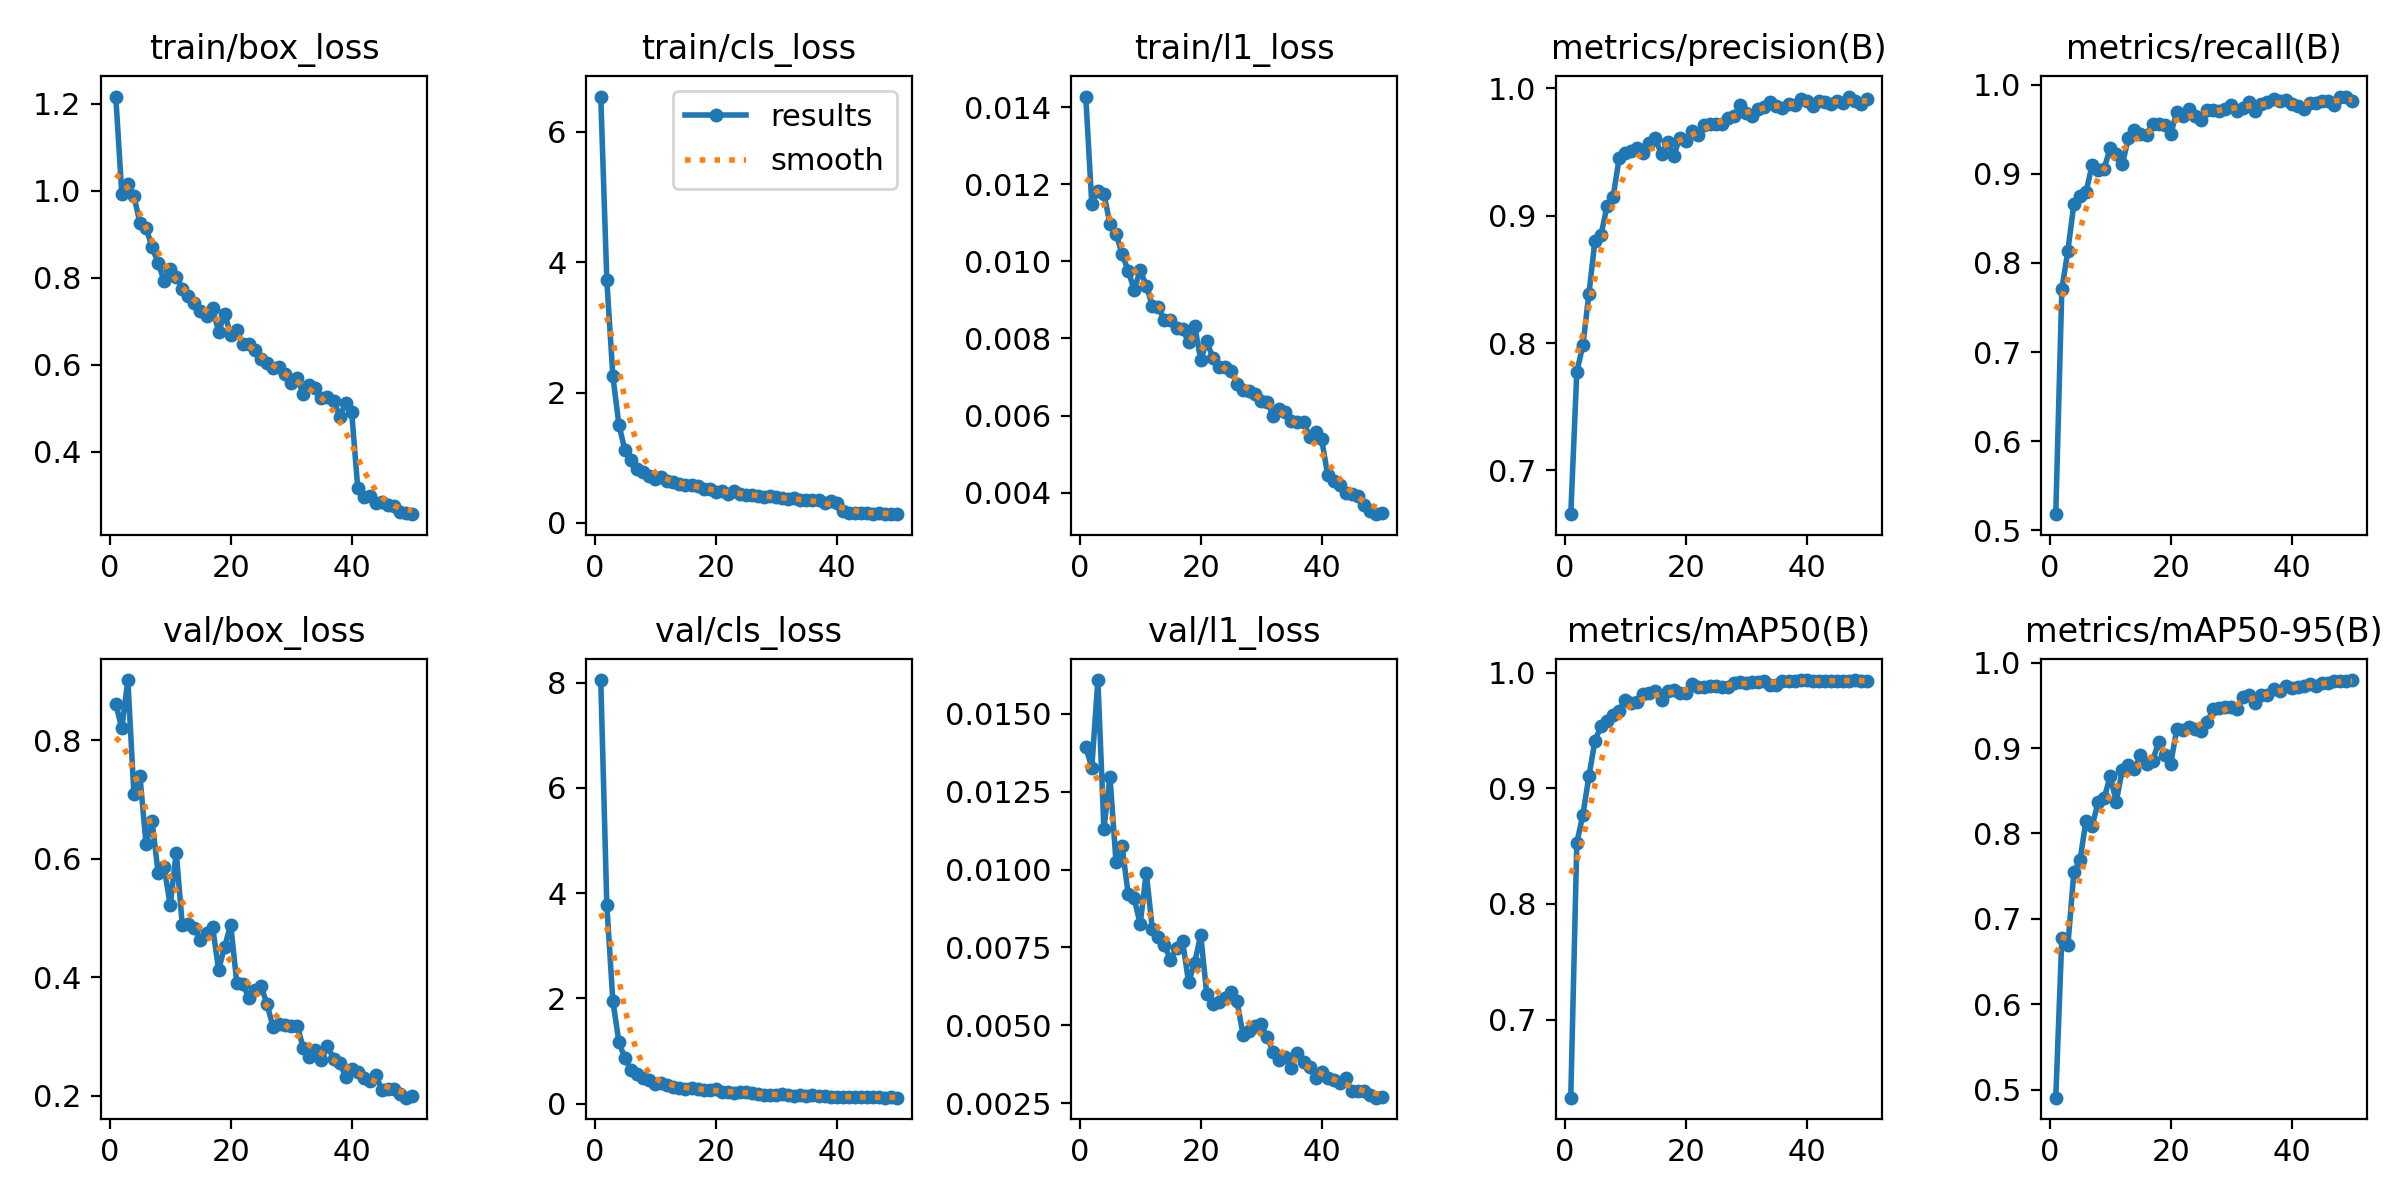
\includegraphics[width=0.8\textwidth]{images/1stage_ablation_results.png}
    \caption{Trainingsmetriken des einstufigen Objektdetektors.}
    \label{fig:ablation_1stage_train}
\end{figure}

\begin{figure}[H]
    \centering
    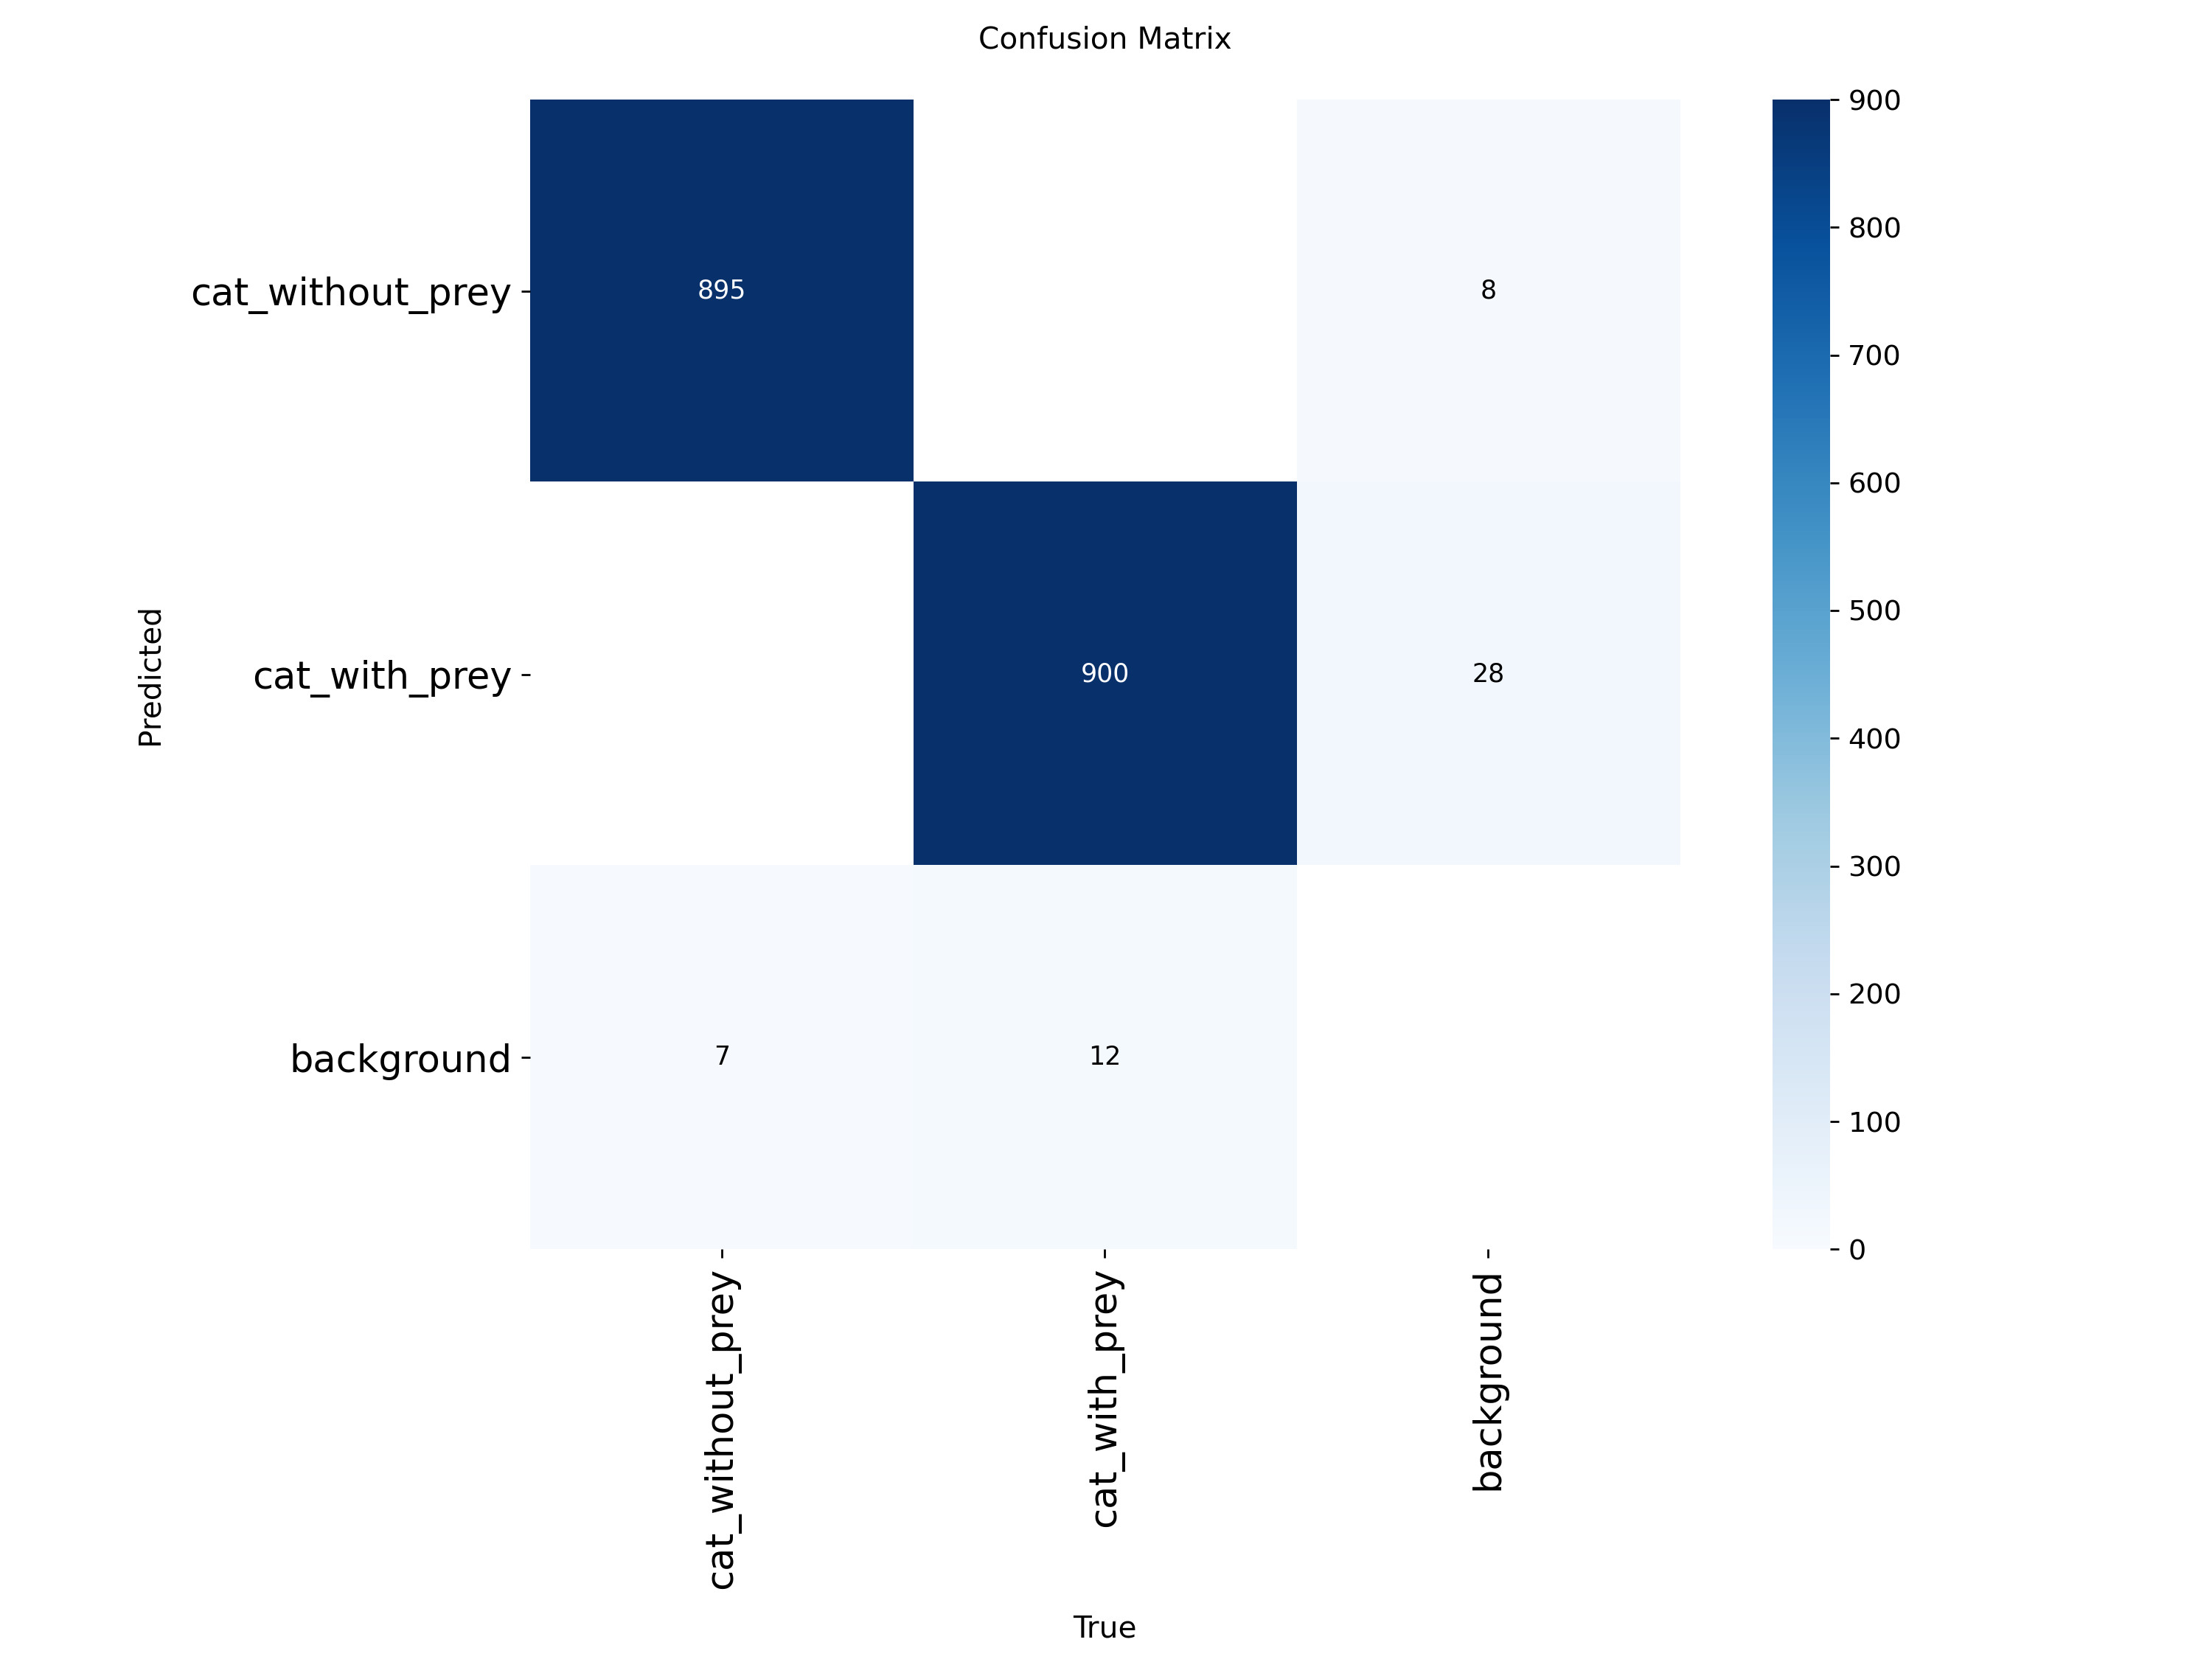
\includegraphics[width=0.7\textwidth]{images/1stage_ablation_confusionmatrix.png}
    \caption{Konfusionsmatrix des einstufigen Objektdetektors auf den Validierungsdaten.}
    \label{fig:ablation_1stage_conf}
\end{figure}


Um die Modelle isoliert zu vergleichen, wurde der Zustandsautomat wieder deaktiviert (\texttt{history\_length=1}). Dabei wurde evaluiert wie viele Sicherheits- und Komfortfehler beide Systeme trafen, sowie wie viele Katzen insgesamt im Video übersehen wurden.
Zusätzlich werden beide Systeme mit dem Zustandsautomaten in der finalen Konfiguration (Zeitfenster von 20 Einzelbildern, Schwellenwert 0,3) ausgewertet. Tabelle~\ref{tab:ablation_1stage} zeigt die Ergebnisse beider Varianten.

\begin{table}[H]
    \centering
    \begin{tabular}{lrrrr}
        \toprule
        & \multicolumn{2}{c}{Ohne Zustandsautomat} & \multicolumn{2}{c}{Mit Zustandsautomat} \\
        \cmidrule(lr){2-3}\cmidrule(lr){4-5}
        Metrik & Zweistufig & Einstufig & Zweistufig & Einstufig \\
        \midrule
        Sicherheitsfehler & 17,3\,\% & 10,1\,\% & 1,6\,\% & 10,6\,\% \\
        Komfortfehler & 20,5\,\% & 62,1\,\% & 4,1\,\% & 30,5\,\% \\
        Präzision & 0,892 & 0,748 & 0,980 & 0,857 \\
        Trefferquote & 0,828 & 0,899 & 0,984 & 0,894 \\
        F1-Maß & 0,859 & 0,817 & 0,982 & 0,875 \\
        Übersehene Katzen & 4,3\,\% & 6,5\,\% & 4,3\,\% & 6,5\,\% \\
        Durchgelassene Beute & 10 von 10 & 10 von 10 & 3 von 10 & 2 von 10 \\
        Entscheidungszeit (sauber) & 0,00\,s & 2,54\,s & 0,67\,s & 3,02\,s \\
        \bottomrule
    \end{tabular}
    \caption{Vergleich des zweistufigen Systems (Detektion und Segmentierung) mit dem einstufigen Objektdetektor, ohne Zustandsautomat (Zeitfenster von einem Einzelbild, Schwellenwert 0,5) und mit Zustandsautomat (Zeitfenster von 20 Einzelbildern, Schwellenwert 0,3).}
    \label{tab:ablation_1stage}
\end{table}

Das einstufige System übersieht mit 6,5\,\% mehr Katzen als der Gesichtsdetektor des zweistufigen Systems (4,3\,\%). Der deutlichste Unterschied zeigt sich beim Komfortfehler: Ohne Zustandsautomat ist die Klappe in 62,1\,\% der Einzelbilder mit sauberen Katzen gesperrt, mit Zustandsautomat in 30,5\,\%. Der einstufige Detektor ordnet saubere Katzen häufig der Klasse \glqq Katze mit Beute\grqq\ zu. Dadurch erreicht er ohne Zustandsautomat zwar einen geringeren Sicherheitsfehler als das zweistufige System, dies geht jedoch zulasten der sauberen Katzen. Mit Zustandsautomat lässt das einstufige System in zwei von zehn Videos Beute durch, das zweistufige System in drei. Der Sicherheitsfehler des einstufigen Systems ist mit 10,6\,\% jedoch mehr als sechsmal so hoch wie jener des zweistufigen Systems (1,6\,\%). Das F1-Maß des zweistufigen Systems liegt mit 0,982 deutlich über jenem des einstufigen Systems (0,875). Zudem benötigt das einstufige System im Mittel 3,02~Sekunden bis zur Freigabe einer sauberen Katze und überschreitet damit die Entscheidungszeit von drei Sekunden.

\subsection{Graustufen gegenüber Farbbildern}
Da die Kamera bei Dunkelheit auf Infrarot-Nachtsicht umschaltet, arbeitet das System durchgehend auf Graustufenbildern. In dieser Studie wird ein auf Graustufenbildern trainiertes System mit einem auf Farbbildern trainierten System verglichen, getrennt nach Tag- und Nachtaufnahmen.
Beide Segmentierungsmodelle besitzen dieselbe Architektur (YOLO26n-seg) und werden mit denselben Trainingsdaten trainiert. Das Farbmodell erhält dabei die ursprünglichen Farbbilder, das Graustufenmodell die in Graustufen umgewandelten Bilder. Der Gesichtsdetektor und der Zustandsautomat (Zeitfenster von 20 Einzelbildern, Schwellenwert 0,3) bleiben in beiden Konfigurationen unverändert. Die Tagaufnahmen umfassen sechs, die Infrarot-Aufnahmen vier Videopaare. Tabelle~\ref{tab:ablation_gray} zeigt die Ergebnisse.

\begin{table}[H]
    \centering
    \small
    \begin{tabular}{lrrrrrr}
        \toprule
        & \multicolumn{2}{c}{Tag} & \multicolumn{2}{c}{Infrarot} & \multicolumn{2}{c}{Gesamt} \\
        \cmidrule(lr){2-3}\cmidrule(lr){4-5}\cmidrule(lr){6-7}
        Metrik & Grau & Farbe & Grau & Farbe & Grau & Farbe \\
        \midrule
        Sicherheitsfehler & 1,9\,\% & 4,4\,\% & 1,2\,\% & 5,6\,\% & 1,6\,\% & 4,9\,\% \\
        Komfortfehler & 6,8\,\% & 1,3\,\% & 0,0\,\% & 0,0\,\% & 4,1\,\% & 0,8\,\% \\
        Präzision & 0,967 & 0,994 & 1,000 & 1,000 & 0,980 & 0,996 \\
        Trefferquote & 0,981 & 0,956 & 0,988 & 0,944 & 0,984 & 0,951 \\
        F1-Maß & 0,974 & 0,975 & 0,994 & 0,971 & 0,982 & 0,973 \\
        Durchgelassene Beute & 2 von 6 & 2 von 6 & 1 von 4 & 2 von 4 & 3 von 10 & 4 von 10 \\
        Entscheidungszeit (Beute) & 0,19\,s & 0,94\,s & 0,03\,s & 0,75\,s & 0,13\,s & 0,86\,s \\
        \bottomrule
    \end{tabular}
    \caption{Vergleich des Segmentierungsmodells für Graustufenbilder mit dem Segmentierungsmodell für Farbbilder, getrennt nach Tag- und Infrarot-Aufnahmen.}
    \label{tab:ablation_gray}
\end{table}

Bei Tagaufnahmen erreichen beide Modelle ein nahezu gleiches F1-Maß (0,974 gegenüber 0,975). Das Graustufenmodell weist einen geringeren Sicherheitsfehler auf (1,9\,\% gegenüber 4,4\,\%), das Farbmodell einen geringeren Komfortfehler (1,3\,\% gegenüber 6,8\,\%). Bei Infrarot-Aufnahmen liegt keine Farbinformation vor. Hier erzielt das Graustufenmodell einen deutlich geringeren Sicherheitsfehler (1,2\,\% gegenüber 5,6\,\%) und ein höheres F1-Maß (0,994 gegenüber 0,971), während beide Modelle keinen Komfortfehler aufweisen. Zudem sperrt das Graustufenmodell die Klappe bei Katzen mit Beute im Mittel nach 0,13~Sekunden, das Farbmodell erst nach 0,86~Sekunden. Über den gesamten Testdatensatz erreicht das Graustufenmodell das höhere F1-Maß und lässt in drei statt vier Videos Beute durch.
